%% Pattern Analysis and Applications (Springer) submission
%% Built on the official Springer Nature sn-jnl class, sn-basic reference style.
\documentclass[sn-basic]{sn-jnl}

%%, additional packages (sn-jnl already loads geometry, hyperref, fontenc) 
\usepackage{manyfoot}   % sn-jnl calls \DeclareNewFootnote/\SetFootnoteHook but omits the require
\usepackage{threeparttable}
\usepackage{graphicx}
\usepackage{amsmath,amssymb}
\usepackage{xcolor}
\usepackage{booktabs}
\usepackage{multirow}
\usepackage{algorithm}
\usepackage{algpseudocode}
\usepackage{tikz}
\usetikzlibrary{arrows.meta,positioning,fit,backgrounds,calc,shapes.geometric}
\usepackage{pgfplots}
\pgfplotsset{compat=1.18}

% sn-jnl forces every table into a threeparttable+center wrapper, which conflicts
% with our \resizebox-wrapped tabulars and trailing notes. Restore the plain table
% environment the class saved as \tableorg.
\let\table\tableorg
\let\endtable\endtableorg

%%, macros carried over from the manuscript 
\newcommand{\TODO}[1]{{\color{red}\textbf{[TODO: #1]}}}
\newcommand{\Fm}{$F$-measure}
\newcommand{\figplaceholder}[2]{%
  \setlength{\fboxsep}{0pt}%
  \fcolorbox{gray!60}{gray!6}{\begin{minipage}[c][#1][c]{0.98\linewidth}%
  \centering\color{gray!80}\ttfamily\footnotesize
  [\,FIGURE PLACEHOLDER, insert image here\,]\\[4pt]
  \normalfont\itshape #2
  \end{minipage}}}

\raggedbottom

\begin{document}

\title[Adaptive Cross-Scene Foreground Segmentation via Learned Disputed-Pixel Arbitration]{Adaptive Cross-Scene Foreground Segmentation via Learned Disputed-Pixel Arbitration}

\author[1]{\fnm{Sery Gahouidi Junior} \sur{Thierry}}\email{juniorsery00@gmail.com}

\author*[1]{\fnm{Zhe} \sur{Chen}}\email{zhechen@nuaa.edu.cn}

\affil[1]{\orgdiv{College of Computer Science and Technology}, \orgname{Nanjing University of Aeronautics and Astronautics}, \orgaddress{\city{Nanjing}, \postcode{211106}, \country{China}}}

\abstract{Cross-scene video foreground segmentation via supervised--unsupervised model
communication couples two complementary, imperfect sources of evidence: an
unsupervised background model that adapts per scene but drifts on complex dynamics, and
a supervised network accurate on its training distribution but poor on unseen scenes. The model-communication framework of Liang et al.\ combines
the two, but resolves the pixels on which they disagree with a single fixed,
hand-designed rule. We argue that this fixed resolution of the \emph{disputed} pixels
is the framework's central rigidity, and attach a lightweight, context-aware arbiter
that learns to decide, from evidence it already computes, whether to trust
the unsupervised model, the guidance, or the framework's own resolution. Unlike prior
fusion, which either applies a \emph{fixed} rule to such conflicts or \emph{learns}
only a frame-wide combination of homogeneous unsupervised detectors, ours learns the
decision on the heterogeneous disputed set between a supervised and an unsupervised
branch. To separate learning from reinforcement learning specifically, we also train a
capacity-matched supervised control. On CDnet2014, the learned arbiter improves the
re-implemented framework across a full factorial of two CPB representations
(grayscale and RGB) and two guidance backbones (DeepLabV3+ and PSPNet); the benefit
holds across all four of these configurations. A controlled ablation shows the
reinforcement-learning agent significantly outperforms the supervised control in all
four cells. In
zero-shot transfer to LIMU the learned policy generalises to unseen scenes where a fixed
rule cannot, and we characterise where an already-strong guidance branch resists it. It
is plug-and-play, adding a few thousand parameters while leaving both models
unchanged.}

\keywords{Foreground segmentation, Background subtraction, Model communication, Learned arbitration, Reinforcement learning, Cross-scene generalisation}

\maketitle

\section{Introduction}
Foreground segmentation underpins many vision systems, from surveillance to
autonomous driving. It is intrinsically difficult because the appearance of the
background is scene-dependent: illumination change, dynamic textures (water,
foliage), camera jitter, and intermittent motion all break simple statistical
models. Two paradigms dominate. Unsupervised background subtraction adapts online
and needs no annotation but accumulates errors on complex dynamics; supervised
semantic networks are accurate on their training distribution yet degrade on unseen
scenes and require dense labels.

Liang et al.~[1] proposed an elegant model-communication hybrid: a supervised
guidance model (DeepLabV3+~[3] or PSPNet~[4]) supplies a coarse prior that seeds
selective updates for an unsupervised Co-occurrence Pixel-Block (CPB) model~[2],
which then refines the foreground through a three-stage communication procedure
(a block-selection step, a block-swap step applied where the branches disagree, and a
foreground-resemblance test). The framework is data-efficient and cross-scene, but its
decision engine is a static heuristic: the CPB foreground test compares a weighted vote
against a fixed relevance cutoff $\lambda=0.5$, and disagreements between the branches
are resolved by a hand-designed support-block rule. A single static rule cannot be
optimal across the enormous variety of local contexts in a cross-scene benchmark.

Our thesis is that this arbitration should be \emph{learned}, and that it need only
be learned where the two branches actually disagree, the disputed pixels, which
are typically only a small fraction of valid pixels (measured per scene, roughly
$1.5$--$8.5\%$ on cameraJitter and $1.7$--$20.6\%$ on the hardest turbulence scenes,
and below $10\%$ on average). We attach a lightweight, context-aware arbiter to
exactly those pixels and leave the rest of the framework untouched, keeping the
method plug-and-play and computationally negligible while concentrating learning
where the original framework is uncertain. We further ask which learning paradigm
the arbitration requires, and design controlled experiments that separate the
effect of \emph{learned, context-aware} arbitration from the effect of
reinforcement learning specifically.

This framing sharpens how our contribution differs from existing fusion. Semantic
background subtraction and the Liang et al.\ communication framework already
\emph{localise} the disagreement between a supervised and an unsupervised branch, but
resolve it with \emph{fixed}, hand-designed thresholds and precedence rules~[1,\,15].
Conversely, learned fusers train a network to combine the outputs of several
\emph{homogeneous} unsupervised detectors over the \emph{entire} frame, rather than
arbitrating between two heterogeneous sources of evidence~[16]. Among the methods we
surveyed, including mixture-of-experts and selective-prediction approaches (Sec.~2.3),
we are not aware of prior work that \emph{learns} the decision on precisely the
heterogeneous disputed set where a supervised guidance branch and an unsupervised
background model conflict
which is exactly the gap this paper fills, while the recent trend of ever-stronger
foundation-model guidance~[31,\,36,\,37] only makes the question of \emph{how} to
arbitrate between such complementary branches more pressing.

In light of the above, this paper makes the following contributions. First, we
formulate disputed-pixel arbitration as a one-step contextual decision, with a
23-dimensional state summarising the evidence the framework already produces, a
three-way action space (\emph{trust-CPB}, \emph{trust-guidance}, or
\emph{keep-baseline}), and a segment-level soft-$F_1$ reward, and we learn it with
the REINFORCE policy-gradient estimator augmented by a behaviour-cloning auxiliary;
the keep-baseline action preserves the framework's own Stage-2/3 resolution, so the
arbiter never discards the support-block machinery but only overrides it when
confident. Second, we contribute a careful, honest re-implementation of the base
framework as the controlled foundation for these comparisons, documenting the
reconstruction choices we found necessary and reporting transparently where our
reproduction still falls short of the authors' absolute level (Sec.~\ref{sec:repro}).
Third, on
CDnet2014 and under a strict 5-fold scene-disjoint cross-validation protocol (the
scenes partitioned into five folds, with four folds used for training and the held-out
fold for testing) in which every
system is scored on identical held-out pixels, we show that learned arbitration
consistently improves the re-implemented framework across a full $2\times2$ of two
unsupervised CPB representations (grayscale and RGB) and two guidance backbones
(DeepLabV3+ and PSPNet): in the primary RGB\,/\,DeepLabV3+ configuration it raises the
category-mean \Fm{} from $0.540$ to $0.660$ ($+0.120$) with all $11$ categories
improved, and, crucially, the reinforcement-learning agent \emph{beats the
capacity-matched supervised control} in a single-harness head-to-head ($0.660$ vs.\
$0.625$ category-mean). This RL-over-supervised advantage is now \emph{statistically
significant in every one of the four configurations} (paired Wilcoxon over the $53$
held-out scenes, $p$ from $5\times10^{-5}$ to $4\times10^{-4}$), with a strikingly
stable category-mean margin of $+0.037\pm0.002$. The arbiter is \emph{modular}, and the
gain is \emph{base-invariant across the four configurations tested}: the same
improvement, and the same RL-over-supervised ordering, hold for each CPB representation
and guidance backbone, with the arbiter retrained within each configuration.
On the aggregation the original authors report for CDnet (pooled), our full RGB system
under DeepLabV3+ guidance reaches $0.775$, \emph{comparable to} their reported $0.753$;
we give this only as a reference point, \emph{not} a claim of superiority over the
original method, and we build on a weaker reproduced CPB (on the stricter
category-mean we remain below their computable level, which we state plainly in
Sec.~\ref{sec:repro}). Finally,
through a set of controlled analyses, the single-harness head-to-head, a
cross-dataset transfer to the LIMU dataset across the same $2\times2$, and a
guidance-backbone ablation, we locate the source of the improvement in the
\emph{learned} nature of the arbitration and characterise its boundary: the agent
beats the supervised control in transfer in all four configurations and is the best
deployable system under DeepLabV3+, whereas under a PSPNet backbone that is already
strong on the target dataset, simply trusting the guidance becomes hard for any
arbiter to beat. Taken
together, these results demonstrate that it is both possible and beneficial to learn
the disputed-pixel arbitration of a supervised--unsupervised communication
framework, without retraining either underlying model and while leaving the
large majority of pixels (typically more than $90\%$) on which the two branches agree entirely unchanged.

The remainder of this paper is organised as follows. Section~\ref{sec:related}
reviews related work on background subtraction, learned decision fusion, and
reinforcement learning for visual decision making. Section~\ref{sec:method} recalls
the base communication framework and presents the proposed arbiter, its state,
action space, and reward. Section~\ref{sec:exp} describes the experimental protocol
and reports the main result together with the controlled analyses, and includes a
dedicated discussion of the reproduction gap. Section~\ref{sec:conc} concludes.

% ============================================================================
% 
%  SECTION 2, RELATED WORK  (author's expert-reviewed version, inlined)
% 
\section{Related Work}
\label{sec:related}

\subsection{Unsupervised Background Subtraction}
Unsupervised background subtraction methods model the appearance of the scene from
video observations and determine foreground regions from deviations from the
learned background. Classical approaches include parametric pixel-wise models, such
as the adaptive Gaussian mixture model of Stauffer and Grimson~[9], as well as
non-parametric sample-consensus methods such as ViBe~[10] and SuBSENSE~[11]. These
approaches have the important advantage of adapting to scene changes without
requiring manually annotated foreground masks. However, their online adaptation can
also accumulate erroneous observations, particularly in the presence of dynamic
textures, intermittent motion, illumination changes, and other non-stationary
background phenomena.

A different family of background models exploits spatial relationships rather than
treating each pixel independently. The Co-occurrence Pixel-Block (CPB) model~[2]
represents a target pixel using a set of spatially correlated supporting blocks and
detects foreground when the learned intensity relationship between the target and
its supporting background blocks is violated. This spatial representation provides
robustness to local appearance variation and does not require the type of
continuously scheduled model update used by many conventional background
subtraction methods. Nevertheless, once its statistical relationships have been
established, CPB has limited ability to adapt when the selected supporting blocks
become inappropriate for a changing scene, for example when a foreground object
repeatedly occupies a region previously treated as background. The subsequent
model-communication framework of Liang et al.~[1] addresses this rigidity by using
an external supervised model to guide the selection and replacement of CPB
supporting blocks. Our work builds directly on this framework and targets what
remains the governing rigidity of the combined system: how the disagreements
between its two complementary sources of evidence are resolved.

\subsection{Deep and Semantic Segmentation for Foreground Detection}
Deep learning has substantially advanced foreground segmentation by learning
spatial and, in some cases, temporal representations directly from annotated video
data. CNN-based background subtraction methods such as DeepBS~[12] and FgSegNet~[13]
demonstrated that learned representations can achieve very strong foreground
segmentation accuracy, although often under a scene-specific protocol in which the
network is exposed to frames of the target scene. Later work such as BSUV-Net~[14]
and its video-agnostic successor BSUV-Net~2.0~[33] explicitly addressed the harder
setting of background subtraction for \emph{unseen} videos, and more recent
scene-independent methods push cross-scene generalisation further without any
target-scene labels: the zero-shot ZBS~[34] models the background at the instance
level using an open-vocabulary detector, while MUSTAN~[35] exploits multi-scale
temporal context to improve out-of-domain foreground segmentation. Nevertheless,
CNN-based methods remain dependent on the availability and
representativeness of training data, and their performance can deteriorate when the
target scene exhibits characteristics that are poorly represented in the training
distribution. In particular, the cross-scene setting is challenging because
background appearance, camera behaviour, illumination, and object configurations can
vary substantially between scenes.

Semantic segmentation provides another useful source of high-level visual
information. Networks such as PSPNet~[4] and DeepLabV3+~[3] learn object-level
representations and can provide semantic priors even when foreground-specific
annotations are unavailable. When trained on datasets such as ADE20K~[8], these
networks can identify classes that are commonly associated with foreground objects.
More recently, promptable foundation segmenters such as the Segment Anything Model~[31]
provide class-agnostic masks of strikingly high spatial quality, and test-time
adaptation methods~[22,\,32] can adjust a segmentation network to a target distribution
online; both are natural, stronger drop-in replacements for the guidance branch used
here. A fast-growing line of very recent work indeed builds moving-object
segmentation directly on such foundation models by coupling them with motion
cues~[36,\,37], confirming that stronger guidance is increasingly available off the
shelf and that the question of \emph{how} to combine a powerful semantic prior with a
motion/background cue is more pertinent than ever. We deliberately adopt a fixed,
publicly available ADE20K prior rather than a
foundation-model prior, both to remain a faithful reproduction of Liang et al.\ and
because our contribution, learning the arbitration between the two branches, is
orthogonal to, and would only benefit from, a stronger guidance source.
However, semantic segmentation is not equivalent to motion-based foreground
detection: semantic networks primarily describe \emph{what} an image region
represents, whereas background subtraction must additionally determine
\emph{whether} that region constitutes foreground in the current scene and temporal
context. Consequently, semantic predictions can contain both false positives and
false negatives when object identity alone is insufficient to distinguish a moving
foreground object from a static background object.

Several studies have therefore investigated combinations of conventional background
subtraction and semantic information. Semantic background subtraction methods
combine a background model with a semantic branch through predefined decision
mechanisms~[15,\,16]. Liang et al.~[1] substantially generalised this idea by
introducing a bidirectional communication framework in which a supervised
segmentation model provides coarse guidance for the unsupervised CPB model, while
CPB subsequently contributes fine-grained information to the final segmentation.
Their framework lets the guidance prediction steer which background blocks are chosen
and when they are swapped, and then recovers foreground regions by a resemblance test in
feature space. This combination is particularly relevant to our
work because it establishes a complementary relationship between semantic and
statistical evidence rather than requiring either branch to solve foreground
segmentation independently. However, the interaction between the branches remains
governed by predefined rules. Our work retains this complementary architecture but
replaces its fixed arbitration on ambiguous pixels with a learned decision
mechanism.

\subsection{Learned Decision Fusion and Expert Routing}
The problem of deciding which of several competing predictors should be trusted has
been studied extensively in ensemble learning and mixture-of-experts models.
Mixtures of experts introduce a learned gating mechanism that assigns different
inputs to specialised predictors~[17], while sparsely gated mixture-of-experts
architectures further scale this principle by dynamically selecting a subset of
experts for each input~[18]. Related work has also investigated probabilistic
fusion of multiple background classifiers, allowing complementary classifiers to
contribute jointly to the final background decision~[19]. These approaches establish
an important general principle: when different models possess complementary
strengths, a learned decision mechanism can determine which source should dominate
for a particular input.

Our problem is related to this general notion of learned gating, but differs in both
scope and purpose. The proposed arbiter is not a generic ensemble combiner that
independently aggregates several complete segmentation networks. Instead, it is
embedded inside the CPB--guidance communication framework of Liang et al.~[1] and is
invoked specifically where the two existing branches disagree. The decision
mechanism therefore operates on a restricted set of ambiguous pixels rather than
replacing either segmentation model. Moreover, its input is derived from evidence
already produced by the framework, including CPB confidence and support statistics,
guidance information, and local scene context. Finally, the arbiter is trained with
the objective of improving the resulting segmentation quality rather than merely
learning a generic classifier combination rule. The proposed formulation can
therefore be viewed as a specialised, framework-aware gating mechanism whose purpose
is to resolve disagreement between two heterogeneous foreground cues.

\subsection{Cross-Scene Generalisation and Domain Adaptation}
Generalising visual segmentation models from observed scenes to unseen environments
is closely related to domain adaptation and domain generalisation. Methods such as
AdaptSegNet~[20] and CyCADA~[21] address domain discrepancies by learning
representations or output spaces that are more invariant between source and target
domains. Test-time adaptation methods such as Tent~[22] instead adapt a pretrained
model during inference, typically using information from the target distribution
itself. Meta-learning and few-shot segmentation approaches~[23,\,24] provide another
strategy by learning models that can rapidly adapt to a new task or scene from a
small amount of target information.

These approaches differ from the cross-scene setting considered here in an important
respect. The proposed arbiter is trained using source scenes and then applied to
previously unseen scenes without requiring target-scene annotations, target-scene
fine-tuning, or an online adaptation stage. The underlying CPB model remains
scene-specific through its normal background modelling process, while the learned
arbiter captures a more general decision rule for resolving disagreement between CPB
and the supervised guidance model. Furthermore, the arbiter does not attempt to
transform the entire feature distribution of the target scene; it operates only on
pixels for which the two existing segmentation sources provide conflicting evidence.
This restricted intervention reduces the amount of learned behaviour that must
generalise across domains and allows the original communication framework to remain
unchanged elsewhere.

\subsection{Reinforcement Learning for Visual Decision Making}
Reinforcement learning has previously been used to formulate visual processing as a
sequence of decisions rather than as a single feed-forward prediction. Active object
localization with deep reinforcement learning~[25], for example, learns an agent
that iteratively transforms a candidate bounding box to localise an object.
Similarly, ADNet~[26] formulates visual tracking as a sequence of learned actions,
while Han et al.~[6] introduced a reinforcement-learning-based cutting agent for
video object segmentation. The latter is particularly relevant to the present work
because it demonstrates how reinforcement learning can be used to make localised
decisions that progressively influence visual segmentation.

Our formulation differs from these sequential visual decision problems. The proposed
agent does not search for an object, move a bounding box, or modify a region through
a long sequence of actions. Instead, at each disputed pixel, it observes the local
evidence produced by the existing segmentation framework and chooses which available
decision source should be trusted. Consequently, the fundamental learning problem is
substantially more local: each disputed pixel corresponds to a one-step contextual
decision, with no action-induced transition that changes the state of another
disputed pixel. This makes the formulation closer to a contextual bandit, or
equivalently a one-step Markov decision process, than to a long-horizon
sequential MDP. The distinction is important when selecting the learning algorithm:
we therefore employ the policy-gradient estimator REINFORCE~[7], rather than methods
such as PPO~[27] or SAC~[28], which were developed for general sequential decision
problems with longer horizons and explicit temporal credit assignment. The
formulation allows the learned policy to focus specifically on the ambiguous cases
generated by model communication while leaving pixels on which the two branches
agree unchanged.

\medskip
Overall, the literature reveals a progression from independent statistical
background modelling, to supervised and semantic segmentation, and subsequently to
hybrid systems that combine these complementary sources of information. Liang et
al.~[1] provide the closest foundation to our work by demonstrating that supervised
guidance can compensate for the limitations of CPB while CPB can in turn refine the
coarse supervised prediction. However, their communication mechanism ultimately
relies on fixed decision rules. Existing mixture-of-experts and fusion methods
demonstrate the value of learned gating, and reinforcement-learning studies establish
the feasibility of learned visual decision making, but neither line of
work specifically addresses cross-scene, per-pixel arbitration between an
unsupervised CPB model and a supervised guidance model within the Liang
communication framework. Our work addresses this gap by learning a lightweight,
context-aware arbiter that intervenes only on the small subset of pixels where the
two branches disagree, thereby preserving the original communication pipeline while
making its critical arbitration step adaptive rather than fixed.

% ============================================================================
\section{Method}
\label{sec:method}

%  Figure 1: base framework (Liang et al.) schematic 
\begin{figure}[t]\centering
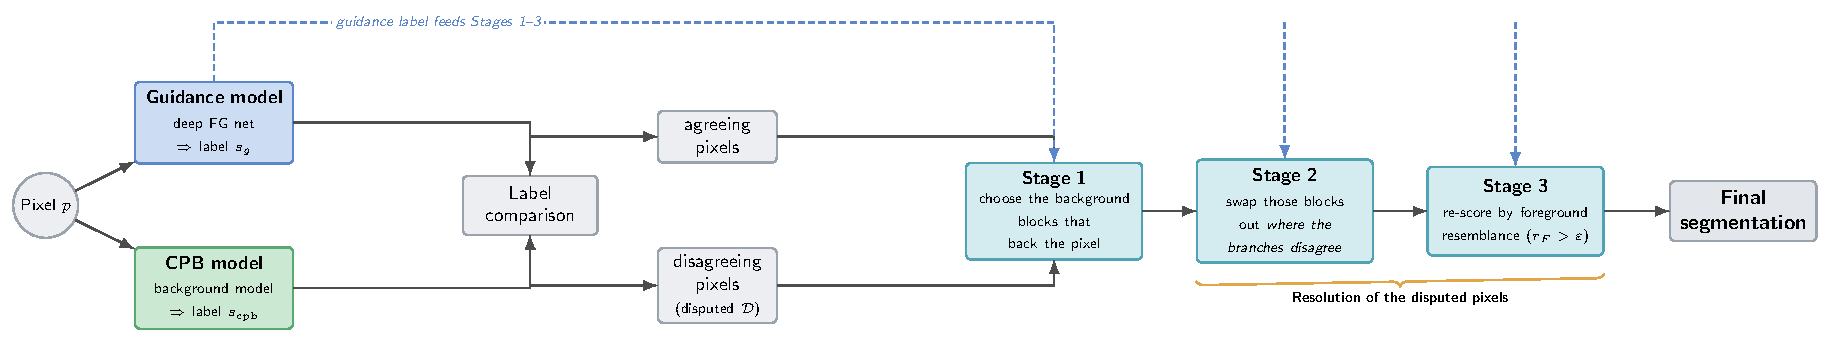
\includegraphics[width=\textwidth]{fig_liang_flow.pdf}
\caption{The base cross-scene segmentation framework of Liang et al.~[1] that we
reproduce, drawn at the level of a single pixel $p$. The pixel receives a supervised
guidance label $s_g$ and an unsupervised CPB label $s_{\text{cpb}}$; a label comparison
sorts pixels into \emph{agreeing} and \emph{disagreeing} (disputed) sets. All pixels then
pass through the three-stage model communication, Stage~1 (choosing the background blocks
that back the pixel), Stage~2 (swapping those blocks out \emph{where the two branches
disagree}), and Stage~3 (re-scoring the pixel by foreground resemblance,
$r_F>\varepsilon$), with the guidance label feeding
every stage. Stages~2--3 are the fixed hand-designed resolution of the disputed pixels
$\mathcal{D}$, applied by a rule that is the same for every scene.}
\label{fig:method}
\end{figure}

%  Figure: our method flow (learned arbiter) 
\begin{figure}[t]\centering
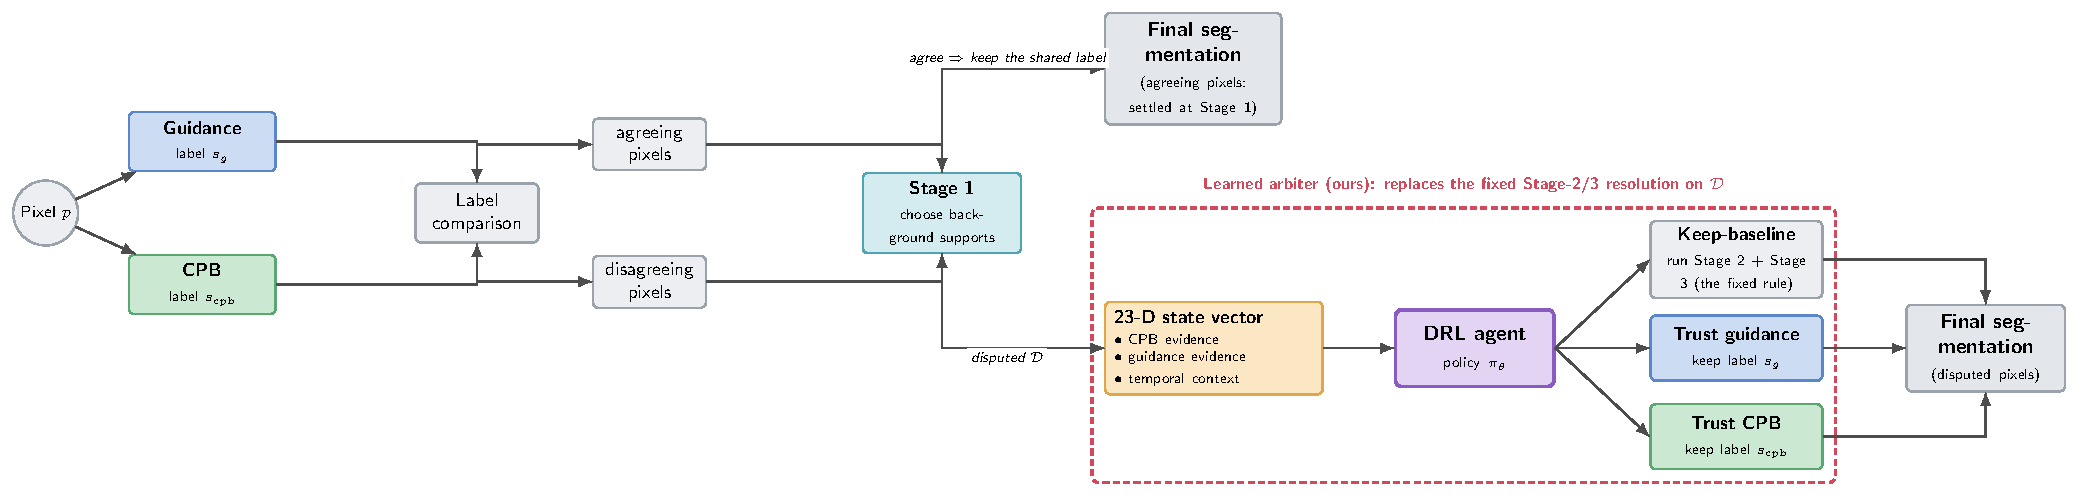
\includegraphics[width=\textwidth]{fig_ours_flow.pdf}
\caption{Our method at the level of a single pixel. The perception is identical to
Fig.~\ref{fig:method}: guidance and CPB label the pixel and a comparison sorts it. Pixels
on which the two branches \emph{agree} keep the shared label (settled at Stage~1). For a
\emph{disputed} pixel we build a 23-D state vector, CPB evidence, guidance evidence and
temporal context, all quantities the framework already computes, and a lightweight DRL
policy $\pi_\theta$ chooses one of three actions: \emph{keep-baseline} (run the original
Stage-2/3 fixed rule), \emph{trust-guidance} (keep $s_g$), or \emph{trust-CPB} (keep
$s_{\text{cpb}}$). Only the fixed Stage-2/3 resolution of $\mathcal{D}$ is replaced (dashed
box); the perception of both branches and the agreeing pixels are untouched.}
\label{fig:ourflow}
\end{figure}

%  Figure: alive per-stage decomposition on a real frame 
\begin{figure}[t]\centering
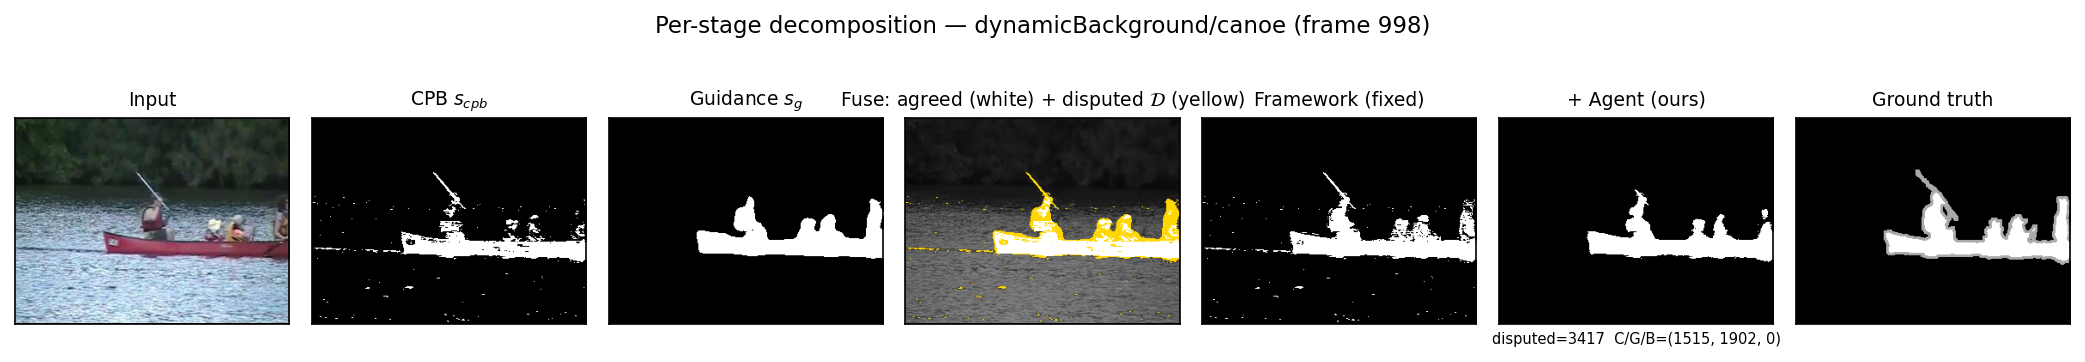
\includegraphics[width=\textwidth]{fig_decomp.png}
\caption{Per-stage decomposition on a real frame (\textit{dynamicBackground/canoe},
frame 998, RGB CPB, DeepLabV3+ guidance, held-out fold). From left to right: the input;
the unsupervised CPB label $s_{\text{cpb}}$, which recovers the boat but also over-fires
across the rippling water (a classic dynamic-background failure); the supervised guidance
$s_g$, which recovers the canoe and paddlers cleanly with almost no water response; the
\emph{Fuse} view, which marks on a dimmed input the \emph{agreed foreground} (white, where
both branches say foreground) and the \emph{disputed set} $\mathcal{D}$ (yellow, where the
two branches disagree, the only pixels the agent acts on, here $3417$ of them,
concentrated on the boat boundary, the paddle, and scattered water speckles); the fixed
framework $s_{\text{fix}}$, which carries water false positives through; the framework with
the learned agent, which suppresses the water and tightens the mask to the boat; and the
ground truth. On this frame the agent's action mix on $\mathcal{D}$ is trust-CPB $1515$ /
trust-guidance $1902$ / keep-baseline $0$. Only pixels in $\mathcal{D}$ are ever changed;
the agreed pixels and both branches' perception are untouched.}
\label{fig:alive}
\end{figure}

\subsection{Framework recap and the dispute set}
\label{sec:recap}
We adopt the CPB $+$ guidance $+$ model-communication framework of~[1,\,2] without
modifying its perception. For a target pixel $p$ with supporting background blocks
$\{Q^{B}_{m}\}_{m=1}^{M}$ ranked by Pearson correlation, CPB scores
foregroundness by a weighted vote over the ``unsteady'' supports and compares it to a
fraction of the total weight:
\begin{equation}
\sum_{m=1}^{M}\gamma_m\,\omega_m \;>\; \lambda \sum_{m=1}^{M}\gamma_m,
\label{eq:cpb}
\end{equation}
where $\gamma_m$ is the correlation weight of support $m$, $\omega_m\in\{0,1\}$
marks whether its intensity relation to $p$ is broken, and
$\lambda=0.5$ is the fixed relevance cutoff. Let $s_{\text{cpb}}(p)$ and
$s_{g}(p)$ be the CPB Stage-1 and guidance labels. The dispute set is
$\mathcal{D}=\{p : s_{\text{cpb}}(p)\neq s_{g}(p)\}$. Agreed pixels are decided by
the original three-stage rule, giving the framework's own label
$s_{\text{fix}}(p)$; our method changes the decision only on $\mathcal{D}$
(Fig.~\ref{fig:alive}).

Importantly, on a disputed pixel $s_{\text{fix}}(p)$ is the output of the
\emph{complete} communication procedure, the Stage-2 block swap
followed by the Stage-3 resemblance test, computed
exactly as in~[1]. Because our keep-baseline action (below) selects
$s_{\text{fix}}$, the arbiter never discards the framework's support-block
machinery; it only decides, per disputed pixel, whether to accept that machinery's
output or to override it with a raw branch label. All pixels the Stage-2/3 machinery
modifies lie within $\mathcal{D}$, so the arbiter and the original communication act
on exactly the same set.

\subsection{Arbitration as a one-step contextual decision}
For each disputed pixel the arbiter observes a context $s_t$ and selects one action
$a_t$; the action determines that pixel's label and does not alter the context of
any other pixel. There is thus no state transition induced by the action, so the
process is a contextual bandit (equivalently, a one-step MDP), not a multi-step MDP.
The reward for a frame is computed from the counts induced by all the frame's
actions simultaneously (below), so it is invariant to the order in which pixels are
processed. This framing is why a policy-gradient estimator without temporal
bootstrapping is the appropriate learner.

\paragraph{State $s_t\in\mathbb{R}^{23}$.}
The state summarises the local evidence around a disputed pixel using only
quantities the framework already computes, in three groups (Table~\ref{tab:state}):
CPB evidence (the continuous score $\sum\gamma_m\omega_m/\sum\gamma_m$, live-support
count, a short temporal window of the CPB score including a persistence statistic,
and local spatial statistics including connected-component blob size), guidance
evidence (probability, confidence, and geometry relative to confident guidance
regions), and generic context (motion, edge, texture, contrast).

%  Table: the 23-D state 
\begin{table}[t]\centering
\caption{The 23-dimensional arbitration state $s_t$. All features derive from
quantities the framework already produces; no new perception is added.}
\label{tab:state}
\small
\begin{tabular}{p{0.22\textwidth} p{0.5\textwidth} p{0.2\textwidth}}
\toprule
group & features & intuition\\
\midrule
CPB evidence (11) & score, margin, live-support count, 1-step $\Delta$score, window mean/std/slope/persistence, spatial-context mean/std, connected-component blob size & foregroundness and confidence of the unsupervised vote; object vs.\ flicker\\
Guidance (7) & label, probability, confidence, soft disagreement, distance-in/out, local density, distance-to-confident-region & strength and geometry of the semantic prior\\
Context (5) & motion, edge, texture, contrast, guidance reliability & generic scene cues\\
\bottomrule
\end{tabular}
\end{table}

\paragraph{Action $a_t\in\{0,1,2\}$.}
Three discrete actions resolve the dispute (Fig.~\ref{fig:ourflow}): $0=$ trust CPB
($s_{\text{cpb}}$), $1=$ trust the guidance ($s_g$), $2=$ keep the framework's own
decision ($s_{\text{fix}}$). Action $2$ everywhere reproduces the original framework
exactly, so the policy departs from the reference only when it expects to help.

\paragraph{Reward.}
Because the \Fm{} is non-differentiable in the discrete per-pixel decisions, we
optimise it directly through the reward. For a frame with running counts
$(TP,FP,FN)$ under the agent's mask we use the marginal contribution of each pixel
to the scene soft-$F_1$,
\begin{equation}
w_{tp}=\tfrac{2(FP+FN)}{(2TP+FP+FN)^2},\quad
w_{pen}=\tfrac{2\,TP}{(2TP+FP+FN)^2},
\end{equation}
assigning $+w_{tp}$ to a true positive and $-w_{pen}$ to a false positive/negative
(normalised), plus small shaping terms that reward fixes (correcting a pixel the
static rule got wrong), penalise breaks (harming a pixel it got right), and add a
confidence term. The reward is masked by the CDnet region of interest, and the
advantage is centred by \emph{this frame's} own mean reward (a per-frame baseline),
which removes a bias a global moving-average baseline induces on low-reward scenes.
Because this baseline is the mean over the frame's disputed pixels, any single action's
influence on it is $O(1/|\mathcal{D}|)$ and negligible for the disputed-set sizes here;
it therefore acts as a variance-reduction control variate rather than a strictly
action-independent baseline.

\paragraph{Policy, training, and the behaviour-cloning auxiliary.}
The policy $\pi_\theta$ is a compact network ($23\!\rightarrow\!64\!\rightarrow\!64
\!\rightarrow\!3$) trained with REINFORCE. On each dispute exactly one primitive
side matches the ground truth; we add a behaviour-cloning (BC) auxiliary that
supervises the policy toward that side, whose weight is linearly annealed
from $1.0$ down to $0.2$ over training. The BC signal injects the (largely separable) arbitration cue
that pure REINFORCE extracts slowly, while the reward retains the freedom to defer
to the framework where the rule inverts. A patch-CNN policy variant that additionally
reads a local window of three maps was implemented but \emph{disabled} for the
reported agent because it was slower to train and did not improve accuracy; the agent
therefore uses the same scalar inputs as the supervised control;
checkpoints are selected by a harm-aware criterion (mean category gain penalised by
the worst category). Algorithm~\ref{alg:train} summarises the full training loop.

\begin{algorithm}[t]
\caption{Training the disputed-pixel arbiter (REINFORCE with a behaviour-cloning auxiliary).}
\label{alg:train}
\begin{algorithmic}[1]
\Require training frames; policy $\pi_\theta$; BC weight schedule $\beta$ ($1.0\!\rightarrow\!0.2$); learning rate $\eta$
\Ensure trained policy $\pi_\theta$
\For{each training iteration}
  \State sample a frame; run CPB and guidance to obtain labels $s_{\text{cpb}},\, s_g$
  \State $\mathcal{D} \gets \{\, p : s_{\text{cpb}}(p) \neq s_g(p) \,\}$ \Comment{disputed set}
  \ForAll{$p \in \mathcal{D}$}
     \State $x_p \gets \mathrm{state}(p)$ \Comment{$23$-dimensional feature vector}
     \State sample $a_p \sim \pi_\theta(\cdot \mid x_p)$, \; $a_p \in \{\text{trust-CPB},\,\text{trust-guidance},\,\text{keep-baseline}\}$
  \EndFor
  \State form the frame mask: apply $\{a_p\}$ on $\mathcal{D}$, keep the shared label on agreed pixels
  \ForAll{$p \in \mathcal{D}$}
     \State $r_p \gets$ marginal contribution of $p$ to the frame soft-$F_1$ \Comment{$+w_{tp}$ / $-w_{pen}$, Eq.~(2), plus shaping}
  \EndFor
  \State $b \gets \tfrac{1}{|\mathcal{D}|}\sum_{p\in\mathcal{D}} r_p$ \Comment{per-frame advantage baseline}
  \State $a^{\star}_{p} \gets$ oracle action for each $p \in \mathcal{D}$ \Comment{the side matching the ground truth}
  \State $g \gets \displaystyle\sum_{p\in\mathcal{D}} (r_p-b)\,\nabla_\theta \log \pi_\theta(a_p\mid x_p) \;+\; \beta \!\sum_{p\in\mathcal{D}} \nabla_\theta \log \pi_\theta(a^{\star}_{p} \mid x_p)$
  \State $\theta \gets \theta + \eta\, g$; \quad anneal $\beta$
\EndFor
\end{algorithmic}
\end{algorithm}

\subsection{A three-way supervised arbiter as control}
\label{sec:control}
To test whether the \emph{learned nature}, rather than reinforcement learning
specifically, drives the gain, we train a capacity-matched supervised classifier
on the identical signal and the identical \emph{three-way} action space
$\{$trust-CPB, trust-guidance, keep-baseline$\}$. Its target is the oracle action
per disputed pixel: keep-baseline whenever the framework's own decision already
matches the ground truth, otherwise the correct primitive branch. Sharing the
agent's action set, and in particular the keep-baseline action, is what makes
the supervised-vs-RL comparison fair: a two-way control lacking keep-baseline would be
forced to overwrite every disputed pixel with a raw branch, discarding the framework's
own reliable resolution on the many disputes where it is already correct. The control
shares the policy's inputs, effective action set, and training scenes, differing
only in the learning paradigm.

% ============================================================================
\section{Experiments}
\label{sec:exp}

\subsection{Datasets, protocol, and metrics}
\label{sec:protocol}
We evaluate primarily on CDnet2014 (11 categories, 53 scenes) and study
cross-dataset transfer on LIMU. CPB models are trained per scene on the first 400
frames; the guidance is DeepLabV3+ with public ADE20K weights (PSPNet is used for
the backbone ablation), not fine-tuned on the evaluation data. The arbiters are
evaluated with 5-fold scene-disjoint cross-validation: the 53 scenes are partitioned
into five folds, and the policy/classifier is trained on four folds and tested on the
held-out fold, so \emph{no test scene is seen in training} and every scene is tested
exactly once across the folds. (A full leave-one-scene-out protocol would require $53$
folds, which is computationally impractical on our CPU-only setup; the five-fold
grouping preserves the no-leakage property at a fraction of the cost.)
We report three aggregations: category-mean (macro over the 11 categories, the
official CDnet metric, which is our primary internal number), scene-mean (macro over
scenes), and pooled (micro-average over all pixel counts). Matching the reference's
aggregation per table is essential to an honest comparison. The exact aggregation
Liang et al.\ use for their ``Overall'' column is not stated in their paper, so we
reconstruct it from their own per-category cells: their published CDnet ``Overall''
($0.753$ for CPB\,+\,DeepLabV3+, $0.772$ for PSPNet) does \emph{not} equal the
arithmetic mean of their $11$ reported categories (that computable category-mean is
$0.771$), but is consistent with a \emph{pooled} micro-average over pixel counts; their
LIMU ``Overall'' ($\approx0.793$), by contrast, is consistent with the \emph{scene-mean}
over the three LIMU scenes. For a reference numerical comparison we therefore report pooled
\Fm{} alongside their CDnet number and scene-mean alongside their LIMU number, while the
standard category-mean remains our \emph{primary} metric. Because the exact aggregation
formula underlying their published numbers is not stated, these comparisons to Liang et
al.\ should be read as reference points rather than as a claim that our evaluation
exactly reproduces their scoring protocol; our load-bearing claims are the controlled,
identical-pixel deltas within our own pipeline, which are independent of this ambiguity.
This distinction is not cosmetic: on LIMU it can invert the sign of a comparison
(Sec.~\ref{sec:transfer}). Following
CDnet, hard shadow ($50$) counts as background and unknown regions ($85/170$) are
excluded. Key parameters follow Liang et al.: $\eta=2.5$, $\sigma=0.8$,
$\mathrm{REF}=20$, block-background threshold $=7$ foreground pixels of $64$,
$\lambda=0.5$, with \emph{no} post-processing.

\paragraph{On aggregation and cross-validation.}
Because our arbiter is a \emph{cross-scene learned} component, cross-validation is
required: the arbiter must be tested on scenes it did not train on. This differs from
the base framework of~[1], which has no cross-scene learned component (its CPB is
trained per scene), and therefore reports all scenes directly without folds. We
report the full-CV category-mean over all scenes; we do \emph{not} report a
best-fold number, which would be a form of test-set selection.

\paragraph{Implementation details (for reproducibility).}
CPB models are trained per scene on the first $400$ frames and then frozen; the
foreground test uses the full-block (all-$64$) steady/unsteady statistic and the
paper-faithful Stage-2 replacement, with $\eta=2.5$, $\sigma=0.8$, $\mathrm{REF}=20$, a
block-background threshold of $7$ foreground pixels of $64$, a per-support scale floor of
$6$, $\lambda=0.5$, and no post-processing; the grayscale and RGB variants differ only in
the number of CPB channels. Guidance is a public DeepLabV3+ (or PSPNet for the backbone
study) with ADE20K weights, not fine-tuned; the soft guidance probability is the sum of
the twelve ADE20K foreground-class channels. The arbiter is a scalar three-way policy
($23\!\rightarrow\!64\!\rightarrow\!64\!\rightarrow\!3$, the patch-CNN branch disabled)
trained with REINFORCE under a per-frame advantage baseline and a segment-level
soft-$F_1$ reward (fix/break/confidence shaping weights $0.5/0.5/0.05$), plus a
behaviour-cloning auxiliary linearly annealed from $1.0$ to $0.2$; optimisation uses Adam
at learning rate $3\times10^{-4}$, $8$ frames per update, gradient-norm clipping at $1.0$,
entropy annealed from $0.01$ to $0.003$, a keep-baseline bias init of $1.5$, and $20{,}000$
steps per fold. Checkpoints are selected by a harm-aware criterion (mean category gain
penalised by the worst category) on a validation set carved one scene per category from
the training folds. The capacity-matched supervised control shares the identical $23$-D
input, three-way action space, and training folds, and is trained by class-balanced
cross-entropy on the per-pixel oracle action. Evaluation uses a $60$-frame uniform sample
within each scene's temporal ROI, scored at native ground-truth resolution; we validated
this sampling against full-sequence scoring (the CPB category-mean over the $60$-frame
sample matches the all-frames value to within $0.003$), so the sample is representative of
the whole scene. All runs use
a fixed seed ($1234$) and the same $5$-fold scene-disjoint partition. Experiments
run on CPU (PyTorch, OpenCV, MMSegmentation); we will release the code, configurations,
and trained checkpoints. In terms of cost, the arbiter is a $23\!\rightarrow\!64\!\rightarrow\!64\!\rightarrow\!3$
MLP ($\approx6$k parameters) evaluated by a single forward pass on only the disputed
pixels ($<10\%$ of the frame on average); its inference cost is therefore negligible
next to the CPB and guidance passes it arbitrates, and it adds no parameters to either
underlying model.

\subsection{The reproduction gap, in detail}
\label{sec:repro}
Because our contribution is measured \emph{relative} to a reproduced base framework, the
fidelity of that reproduction deserves an honest discussion. In short: the gap to the
authors' published numbers is component-level, lies mainly in the unsupervised CPB rather
than in the communication logic, and is closed by the learned arbiter on the authors' own
metric.

\paragraph{Fidelity.} Two details most affect fidelity. First, the CPB steady/unsteady
test: our reconstruction compares the target pixel against the \emph{entire} $8\times8$
support block (satisfied only when all $64$ pixels agree), our reading of the
matrix-valued condition in~[1], whose code is not public. An earlier block-\emph{average}
port is far more permissive and floods dynamic-background and turbulence scenes with false
positives; restoring the full-block rule recovers the authors' qualitative behaviour (on
LIMU \textit{LightSwitch} the framework rises from $\approx0.42$ to $\approx0.78$, matching
their $0.769$). Second, parameterisation: we use Liang et al.'s settings ($\eta=2.5$,
$\sigma=0.8$, $\mathrm{REF}=20$, block-background threshold $7/64$) with \emph{no}
post-processing, so the reproduced system is theirs and not a variant.

\paragraph{The gap is component-level, mainly on the CPB side.}
Comparing on the authors' aggregation (pooled \Fm{}), our faithful framework reaches
$0.57$ versus their $0.753$. The \emph{guidance} is close ($\approx0.62$ vs.\
$\approx0.68$; in fact stronger than theirs on cameraJitter, thermal and badWeather, its
deficits confined to turbulence and intermittent motion, intrinsic limits of
single-frame segmentation). The dominant deficit is the \emph{CPB itself} ($\approx0.42$,
RGB $0.426$ measured, vs.\ $0.63$); our metric harness is verified by reproducing standard
baselines from the authors' own rows (GMM $0.570$ vs.\ $0.571$; SuBSENSE $0.738$ vs.\
$0.741$). A weak CPB caps the whole pipeline, which is why the authors' bare CPB ($0.63$)
can exceed our full framework ($0.57$). Crucially, the learned arbiter closes this on the
authors' metric: our full RGB\,/\,DeepLabV3+ system reaches pooled $0.775>0.753$. We do
not overstate this, on the stricter category-mean we remain below their computable
$0.771$ (the weaker public guidance and structurally hard categories such as turbulence
and PTZ), but on the aggregation they report, the component-level shortfall does not
carry through to the delivered system.

%  Figure: error maps (under-detection signature) 
\begin{figure}[t]\centering
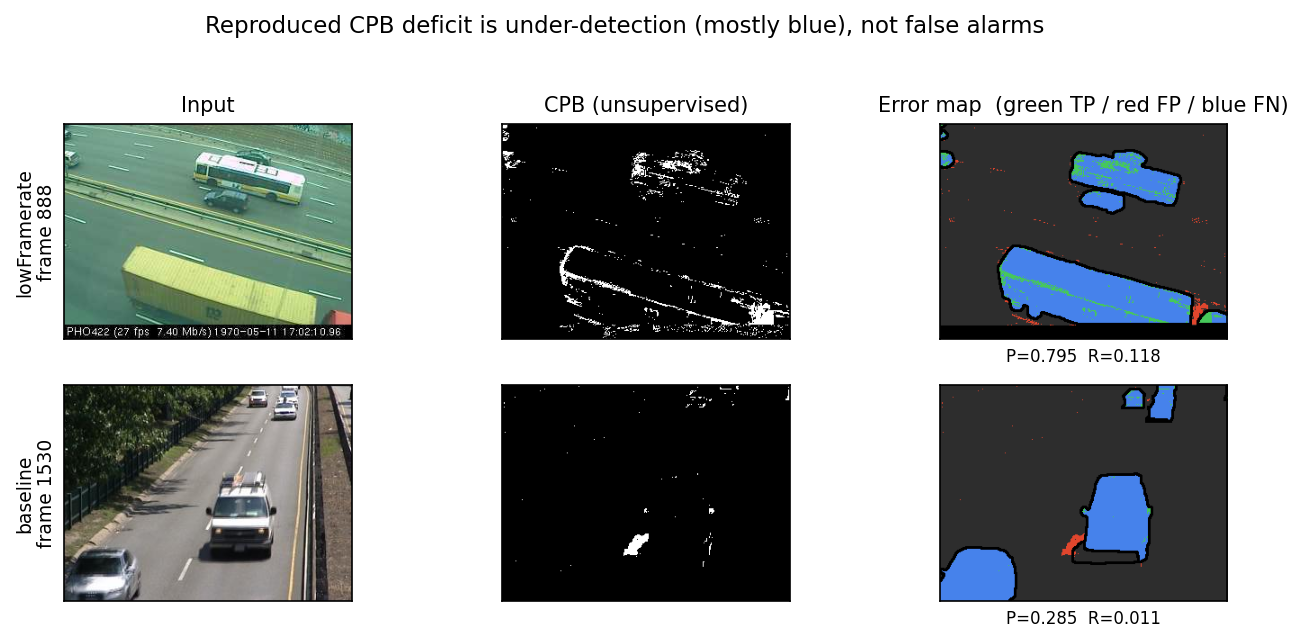
\includegraphics[width=\textwidth]{fig_errormaps.png}
\caption{The reproduced CPB deficit is \emph{under-detection}, not false alarms.
Per-frame error maps of the pure unsupervised CPB for two hard scenes (green $=$ true
positive, red $=$ false positive, blue $=$ false negative). Almost all of the lost score
is \emph{blue}, large, slow, or dim foreground that the frozen CPB \emph{misses} 
while red (spurious over-firing) is negligible. On \textit{lowFramerate/turnpike} the
recall collapses to $0.118$ while precision stays moderate ($0.795$); on
\textit{baseline/highway} the frozen CPB misses the foreground almost entirely
(recall $0.011$). In both cases the dominance of blue over red is the tell-tale signature
of an inflated per-support scale $\sigma$: the acceptance band $\eta\sigma$ is too wide
and genuine foreground is absorbed into the background model, rather than the model
over-firing. This is the mechanism diagnosed and partially corrected below.}
\label{fig:errormaps}
\end{figure}

\paragraph{Diagnosing and partially closing the CPB deficit.}
The deficit is one of \emph{under-detection}: the reproduced CPB is consistently
low-recall, and the error maps (Fig.~\ref{fig:errormaps}) show the lost score is almost
entirely missed foreground, not spurious responses. The cause is a too-tolerant
background model: the per-support scale $\sigma$ is estimated by a plain standard
deviation over training frames that on busy scenes already contain moving objects, so the
foreground spikes inflate $\sigma$, the acceptance band $\eta\sigma$ widens, and genuine
foreground is absorbed, exactly the ``training-sample quality'' effect the authors
warn about. That their bare CPB still reaches $0.633$ suggests practical estimation
choices the paper does not spell out (a robust $\sigma$, or cleaner foreground-free
training frames); our from-the-equations reproduction is faithful to the text but not to
those unstated details. Two targeted fixes confirm the diagnosis (Table~\ref{tab:repro}):
a robust median/MAD $\sigma$ estimator raises the framework category-mean from $0.513$ to
$0.540$, and a guidance-reliability gate (which suppresses the Stage-2 deletion of correct
CPB detections when the guidance is near-empty) raises it further to $0.589$ 
recovering about one third of the gap without touching the guidance or the communication
logic.

%  Table: reproduction recovery (diagnosis) 
\begin{table}[t]\centering
\caption{Diagnosing and partially closing the reproduction gap (CDnet2014,
category-mean \Fm{}, all 53 scenes, 30-frame protocol). The deficit is on the CPB
side; a robust $\sigma$ estimator and a guidance-reliability gate recover
$\approx$one third of the gap without touching the guidance or the communication
logic. We nonetheless adopt the \emph{faithful base} for all controlled comparisons
and report these as a validated diagnosis; the learned arbiter recovers more
($+0.120$ category-mean in the primary configuration) than both hand-engineered fixes
combined ($+0.076$).}
\label{tab:repro}
\small
\resizebox{\columnwidth}{!}{%
\begin{tabular}{@{}lc@{}}
\toprule
configuration & category-mean \Fm\\
\midrule
CPB alone (ours) & 0.374\\
guidance alone (ours) & 0.480\\
\midrule
re-implemented framework (faithful base) & 0.513\\
\;\;$+$ robust $\sigma$ (median/MAD) & 0.540\\
\;\;$+$ robust $\sigma$ $+$ guidance-reliability gate & \textbf{0.589}\\
\midrule
Liang et al.\ (CPB $+$ DeepLabV3+)$^{\dagger}$ & 0.771\\
\bottomrule
\end{tabular}}
\\[3pt]
\footnotesize
$^{\dagger}$For an apples-to-apples comparison in this category-mean table we list the
\emph{computable} category-mean $0.771$ (the arithmetic mean of the authors' $11$
published per-category CDnet cells). Their reported ``Overall'' of $0.753$ is instead a
pooled micro-average (see Sec.~\ref{sec:protocol}); the pooled comparison against
$0.753$ is made in Table~\ref{tab:main}.
The gate has a single hyper-parameter (frame guidance-coverage $<0.1\%$ disables the
Stage-2 deletion); results are stable over $[0.02\%,0.1\%]$. Its residual failures
are scenes with accurate-but-sparse guidance, which coverage cannot distinguish from
empty guidance, the case the learned arbiter resolves from confidence instead.
This recoverability diagnostic uses a lighter 30-frame, all-scenes pass; the main
experiments (Sec.~\ref{sec:main}) use the 60-frame, 5-fold scene-disjoint protocol,
under which the same faithful base scores $0.540$.
\end{table}

\paragraph{Why this reinforces, rather than undercuts, the contribution.}
Two points make the gap supportive of our claim. First, our effect is measured
\emph{relative} to the reproduced base, inside the same pipeline and on \emph{identical}
disputed pixels, so any deficiency in the absolute CPB or guidance level is present
equally in the baseline and the arbitrated system and cancels in the difference; the
$+0.11$ to $+0.14$ category-mean improvement is thus invariant to the reproduction level.
Second, the learned arbiter recovers \emph{more} than the two hand-engineered fixes
combined ($+0.120$ vs.\ $+0.076$), without any hand-set threshold: the fixed reliability
gate must judge guidance trustworthiness from a single coverage number and fails on
accurate-but-sparse guidance (e.g.\ \textit{shadow/cubicle}), whereas the arbiter resolves
the same decision per pixel from CPB confidence and local context. The fixes are a
brittle, hand-crafted instance of what the arbiter learns adaptively; we therefore adopt
the faithful base for all comparisons and take the $+0.120$ improvement
(Sec.~\ref{sec:main}) as our load-bearing claim.

\subsection{Main result: learned vs.\ static arbitration on CDnet2014}
\label{sec:main}
Table~\ref{tab:main} is the paper's anchor, and Fig.~\ref{fig:percat} visualises its
per-category structure. Every system shares the same CPB model and the same guidance;
only the resolution of disputed pixels differs. All five systems are scored in a
\emph{single} harness under 5-fold scene-disjoint cross-validation, so every
number in the table is computed on identical held-out pixels. We report the primary
RGB\,/\,DeepLabV3+ configuration here and give the full $2\times2$ over representations
and backbones in Sec.~\ref{sec:backbone} (Table~\ref{tab:backbone},
Fig.~\ref{fig:robust}). Replacing the static
rule with the learned arbiter raises the category-mean \Fm{} from $0.540$ to $0.660$
($+0.120$), with \emph{all $11$ categories improved}. We stress that this static
baseline ($0.540$) is our \emph{faithful} reproduction (Sec.~\ref{sec:repro}) scored
under the main 5-fold, 60-frame protocol, \emph{not} the robust-$\sigma$ variant of
Table~\ref{tab:repro}; the same faithful base reads $0.513$ there only because that
table uses a 30-frame, all-scenes diagnostic protocol, and the robust-$\sigma$ and gate
rows of Table~\ref{tab:repro} are a separate recoverability analysis that enters
\emph{no} controlled comparison. The improvement is also robust
across aggregations, the agent exceeds the static framework on pooled ($0.775$ vs.\
$0.567$, $+0.208$), scene-mean ($0.667$ vs.\ $0.543$, $+0.124$) and category-mean
($+0.120$) alike, and the per-fold category-mean gain measured in the
cross-validation is $+0.138 \pm 0.070$, i.e.\ consistent across folds rather than
driven by a single lucky split. Notably the fixed rule barely helps here: on this
configuration the static framework's pooled \Fm{} ($0.567$) is \emph{below}
guidance-alone ($0.616$), so almost the entire delivered gain is the arbiter's. On the
pooled aggregation the authors report, our full system reaches $0.775$, comparable to
their $0.753$; we present this only as a reference point, \emph{not} a superiority claim,
since the exact aggregation is unspecified and our stricter category-mean remains below
theirs (Sec.~\ref{sec:repro}). The learned arbiter's action mix on held-out scenes
is roughly trust-CPB $0.45$, trust-guidance $0.45$, keep-baseline $0.10$: it exercises
all three actions, and in particular the keep-baseline action is genuinely used. The
\emph{oracle} row is the ceiling of this exact decision problem: on each disputed pixel it
picks the one of the three actions (trust-CPB, trust-guidance, keep-baseline) that matches
the ground truth, while all agreed pixels are frozen at their shared label, so it upper-
bounds what any disputed-pixel arbiter can achieve, and the agreed-pixel errors it cannot
touch are exactly why its ceiling is $0.825$ rather than $1.0$.

%  Table 1: main result 
\begin{table}[t]\centering
\caption{CDnet2014, 5-fold scene-disjoint CV, every scene tested once, identical
held-out pixels, single scoring harness. Primary configuration: RGB CPB, all-64
framework, DeepLabV3+ guidance. Category-mean is the official CDnet metric; pooled is
the aggregation the authors report as ``Overall''.}
\label{tab:main}
\small
\resizebox{\columnwidth}{!}{%
\begin{tabular}{lccc}
\toprule
system & pooled & scene-mean & cat.-mean\\
\midrule
guidance (DeepLabV3+)        & 0.616 & 0.540 & 0.533\\
framework (Liang, static)    & 0.567 & 0.543 & 0.540\\
framework + supervised MLP   & 0.750 & 0.628 & 0.625\\
\textbf{framework + DRL agent (ours)} & \textbf{0.775} & \textbf{0.667} & \textbf{0.660}\\
oracle (ceiling)             & 0.910 & 0.827 & 0.825\\
\midrule
\emph{Liang et al.\ (CPB+DeepLabV3+), pooled} & \emph{0.753} &, & \\
\bottomrule
\end{tabular}}
\\[4pt]
\footnotesize
agent $-$ framework (cat.): $+0.120$; \; MLP $-$ framework (cat.): $+0.085$;\;
agent $-$ MLP (cat.): $+0.035$ (significant, $p=3.9\times10^{-4}$, Wilcoxon).\\
On pooled the full system ($0.775$) exceeds the authors' reported ``Overall''
($0.753$).\\
Per-fold agent category-mean gain: $+0.138 \pm 0.070$ (5 folds), $11/11$ categories
improved.
\end{table}

%  Table 2: per-category 
\begin{table}[t]\centering
\caption{Per-category CDnet2014 category-mean \Fm{} (5-fold, every scene once,
single harness), primary RGB\,/\,DeepLabV3+ configuration: framework vs.\ supervised
MLP vs.\ DRL agent. Sorted by the agent's gain over the framework. The agent improves
the framework in $11/11$ categories and beats the supervised MLP in $9/11$.}
\label{tab:percat}
\small
\resizebox{\columnwidth}{!}{%
\begin{tabular}{lcccc}
\toprule
category & framework & $+$MLP & $+$agent & agent$-$fw\\
\midrule
dynamicBackground        & 0.612 & 0.693 & 0.842 & $+0.230$\\
PTZ                      & 0.135 & 0.403 & 0.359 & $+0.224$\\
shadow                   & 0.719 & 0.911 & 0.926 & $+0.207$\\
intermittentObjectMotion & 0.526 & 0.626 & 0.683 & $+0.157$\\
baseline                 & 0.650 & 0.744 & 0.801 & $+0.151$\\
badWeather               & 0.607 & 0.720 & 0.742 & $+0.135$\\
lowFramerate             & 0.494 & 0.538 & 0.568 & $+0.074$\\
turbulence               & 0.484 & 0.567 & 0.540 & $+0.056$\\
cameraJitter             & 0.727 & 0.681 & 0.763 & $+0.036$\\
nightVideos              & 0.323 & 0.324 & 0.356 & $+0.033$\\
thermal                  & 0.665 & 0.664 & 0.678 & $+0.013$\\
\midrule
\textbf{category-mean}   & \textbf{0.540} & \textbf{0.625} & \textbf{0.660} & $\mathbf{+0.120}$\\
\bottomrule
\end{tabular}}
\end{table}

%  Figure 2: per-category result bar chart (drawn from head-to-head data) 
\begin{figure}[t]\centering
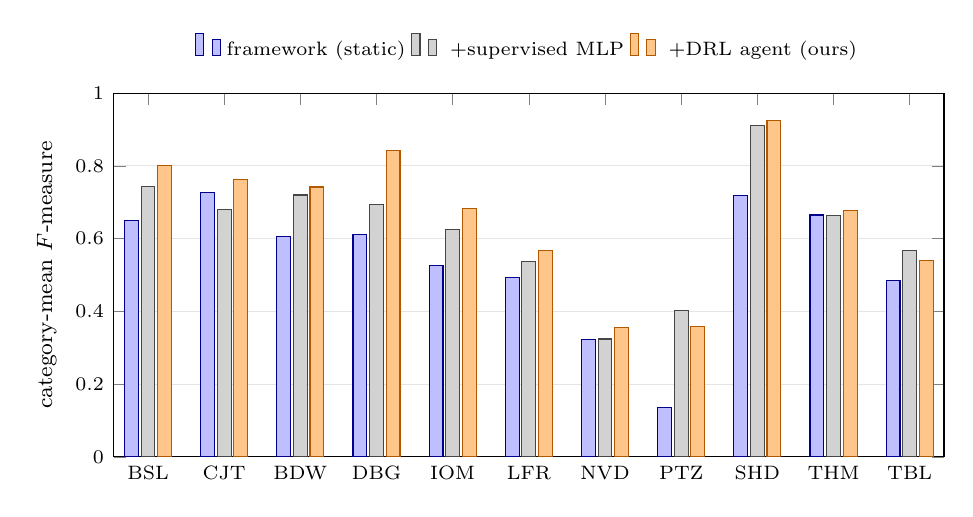
\begin{tikzpicture}
\begin{axis}[
  width=\textwidth, height=6.2cm,
  ybar=1pt, bar width=5pt,
  enlarge x limits=0.045,
  ymin=0, ymax=1.0,
  ymajorgrids, grid style={gray!20},
  ylabel={category-mean \Fm{}}, ylabel style={font=\footnotesize},
  symbolic x coords={BSL,CJT,BDW,DBG,IOM,LFR,NVD,PTZ,SHD,THM,TBL},
  xtick=data, x tick label style={font=\scriptsize},
  y tick label style={font=\scriptsize},
  legend style={font=\scriptsize,at={(0.5,1.06)},anchor=south,legend columns=3,draw=none},
  tick align=inside,
]
\addplot[draw=blue!55!black,fill=blue!25] coordinates {(BSL,0.650)(CJT,0.727)(BDW,0.607)(DBG,0.612)(IOM,0.526)(LFR,0.494)(NVD,0.323)(PTZ,0.135)(SHD,0.719)(THM,0.665)(TBL,0.484)};
\addplot[draw=gray!55!black,fill=gray!35] coordinates {(BSL,0.744)(CJT,0.681)(BDW,0.720)(DBG,0.693)(IOM,0.626)(LFR,0.538)(NVD,0.324)(PTZ,0.403)(SHD,0.911)(THM,0.664)(TBL,0.567)};
\addplot[draw=orange!70!black,fill=orange!45] coordinates {(BSL,0.801)(CJT,0.763)(BDW,0.742)(DBG,0.842)(IOM,0.683)(LFR,0.568)(NVD,0.356)(PTZ,0.359)(SHD,0.926)(THM,0.678)(TBL,0.540)};
\legend{framework (static),\ +supervised MLP,\ +DRL agent (ours)}
\end{axis}
\end{tikzpicture}
\caption{Per-category CDnet2014 category-mean \Fm{} (5-fold scene-disjoint CV,
identical held-out pixels), primary RGB\,/\,DeepLabV3+ configuration from the
single-harness head-to-head. Category codes:
BSL baseline, CJT cameraJitter, BDW badWeather, DBG dynamicBackground, IOM
intermittentObjectMotion, LFR lowFramerate, NVD nightVideos, PTZ, SHD shadow, THM
thermal, TBL turbulence. The learned arbiter (orange) improves the static framework
in \emph{all $11$} categories and beats the supervised MLP in $9/11$; the two
exceptions (PTZ, turbulence) are the categories where the guidance-heavy MLP happens to
help most. On \textit{DBG}, where the branches disagree the most, the agent adds the
largest gain ($+0.230$).}
\label{fig:percat}
\end{figure}

\noindent\emph{Notes on Table~\ref{tab:main}.} All rows come from the single scoring
harness, which trains the supervised control
on the exact scenes each fold's agent saw and scores every system on the same
held-out pixels; the per-fold spread ($\pm0.070$) is measured in the DRL
cross-validation. The spread reflects genuine cross-fold difficulty differences rather
than one anomalous split, the five per-fold category-mean gains are
$+0.112$, $+0.146$, $+0.076$, $+0.084$, and $+0.270$, i.e.\ \emph{every} fold shows a
clear positive gain (the smallest is $+0.076$, none is near zero), with the wide
standard deviation driven by one unusually strong fold rather than by any fold failing.
More importantly, the per-scene test removes the
fold as the unit of analysis: the per-scene agent$-$framework gain is strongly
significant (paired Wilcoxon over the 53 scenes, $p\!\approx\!1.0\times10^{-7}$), as is
the agent$-$MLP gain ($p=3.9\times10^{-4}$); both learned arbiters improve the framework
at $p\!<\!10^{-5}$. The full significance picture across all four configurations is in
Table~\ref{tab:sig}.

Notably the static framework's pooled \Fm{} ($0.567$) is below guidance-alone
($0.616$): on this configuration the fixed rule does not reliably help, and the
arbiter's role is to recover the scenes it collapses. The gain concentrates exactly
where the static rule is weakest (see the per-category breakdown in
Fig.~\ref{fig:percat} and Table~\ref{tab:percat}). Fig.~\ref{fig:qual} shows
representative qualitative results, and Fig.~\ref{fig:dispcmp} contrasts the fixed
rule's and the learned arbiter's \emph{final} masks on a single scene together with
their pixelwise difference.

%  Figure 3: qualitative panels (real, from opus_make_qualitative_agent.py) 
\begin{figure}[t]\centering
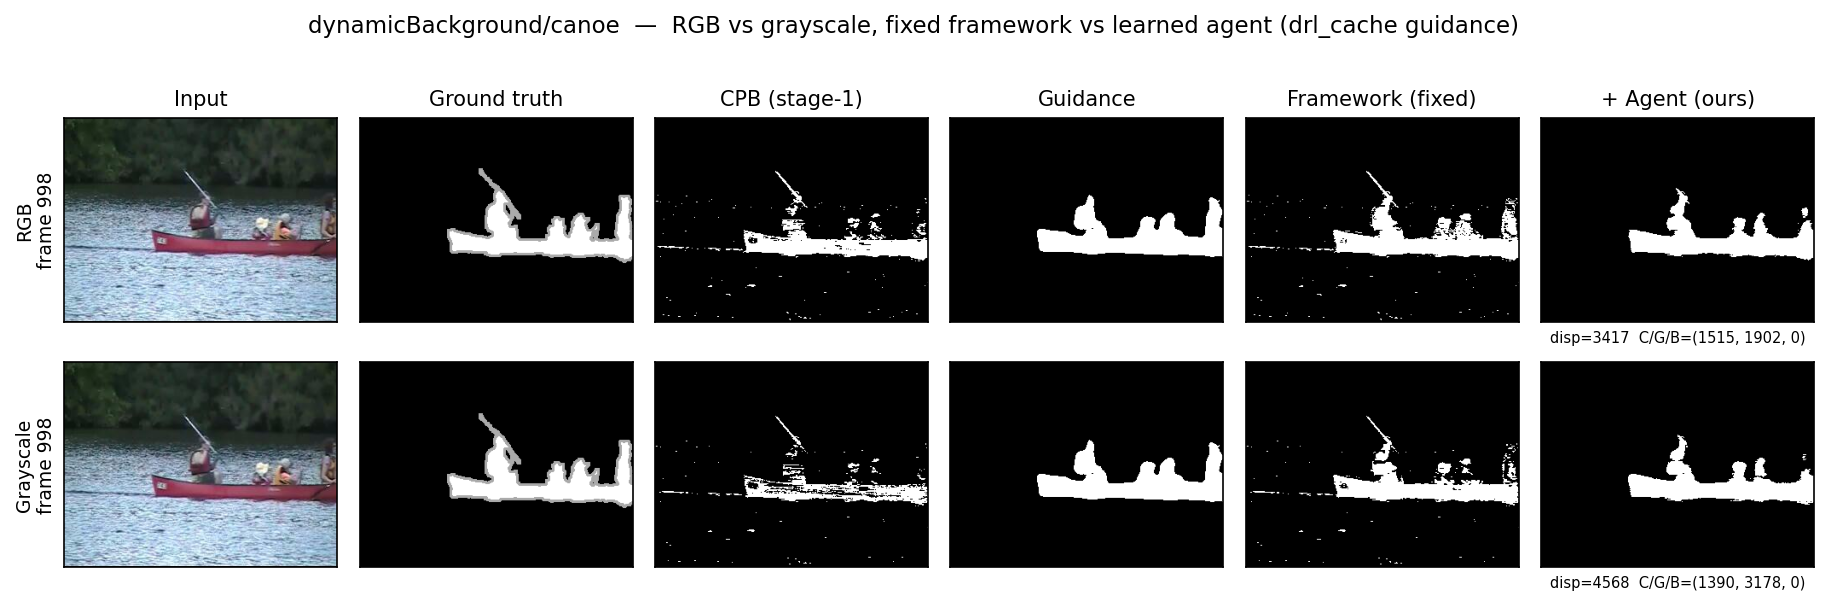
\includegraphics[width=\textwidth]{fig_qualitative_agent_deeplab.png}
\caption{Qualitative comparison on \textit{dynamicBackground/canoe} (frame 998, held-out
fold, DeepLabV3+ guidance), for both CPB representations (top: RGB, bottom: grayscale).
Columns: input, ground truth, CPB Stage-1, guidance, the fixed framework
$s_{\text{fix}}$, and the framework with the learned agent. The unsupervised CPB
over-fires across the rippling water (a classic dynamic-background failure), and the
fixed framework carries much of that water response through, heavily so in grayscale.
The learned agent, acting only on the disputed pixels, suppresses the water and tightens
the mask to the boat and paddlers, visibly closer to the ground truth. The effect is the
same under both representations, illustrating the base-invariance of the contribution;
the agent uses both primitive actions here (trust-CPB and trust-guidance) and never
resorts to a no-op.}
\label{fig:qual}
\end{figure}

%  Figure: same scene, PSPNet backbone (backbone-invariance) 
\begin{figure}[t]\centering
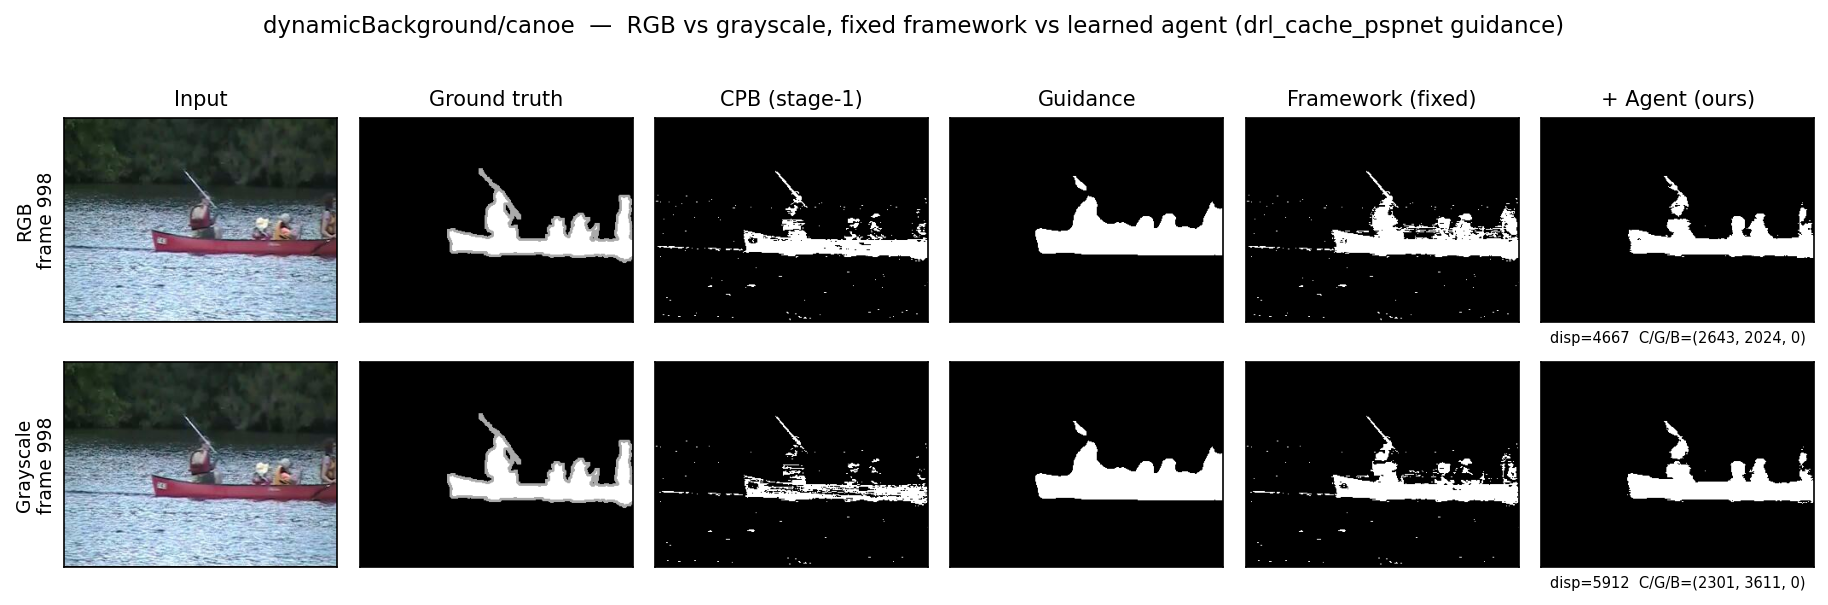
\includegraphics[width=\textwidth]{fig_qualitative_agent_pspnet.png}
\caption{The same scene and frame under a \emph{different} guidance backbone (PSPNet),
columns as in Fig.~\ref{fig:qual}. Although the PSPNet guidance mask differs in shape
from DeepLabV3+, the learned agent again removes the framework's water false positives
and recovers a clean boat under both CPB representations, the arbiter's cleanup is
plug-and-play across the backbone, not tuned to one guidance network's particular
errors. Only disputed pixels are ever changed; the agreed majority is left untouched.}
\label{fig:dispcmp}
\end{figure}

\subsection{Supervised-vs-RL: a single-harness head-to-head}
\label{sec:h2h}
The natural question is whether the improvement requires reinforcement learning or
merely a learned, context-aware decision. To answer it rigorously, rather than by
comparing two separately-run protocols, we evaluate both arbiters in a
\emph{single} scoring harness that trains
the three-way supervised MLP on the exact scenes each fold's agent saw, gives it the
identical 23-D signal and the identical three-way action space, and scores both on
the same held-out pixels. On this common harness in the primary configuration
(Table~\ref{tab:main}) the supervised MLP reaches category-mean $0.625$ ($+0.085$ over
the static framework) and the DRL agent reaches $0.660$ ($+0.120$); the agent therefore
beats the capacity-matched supervised control by $+0.035$ category-mean. The ordering is
consistent across aggregations, the agent also leads on pooled ($0.775$ vs
$0.750$) and scene-mean ($0.667$ vs $0.628$), and it holds in $9$ of the $11$
categories, with the agent's largest margins over the MLP on exactly the categories
the MLP mishandles: \textit{dynamicBackground} ($+0.149$), \textit{cameraJitter}
($+0.082$) and \textit{baseline} ($+0.057$). Relative to the oracle ceiling on disputed
pixels ($0.825$), the agent recovers $42\%$ of the available head-room and the MLP
$30\%$.

Crucially, and unlike an earlier single-configuration run, this RL-over-supervised
advantage is now \emph{statistically significant, and significant in every one of the
four configurations} of the $2\times2$ (paired Wilcoxon over the $53$ held-out scenes;
Table~\ref{tab:sig}): $p=3.9\times10^{-4}$ (RGB\,/\,DeepLabV3+), $1.2\times10^{-4}$
(RGB\,/\,PSPNet), $2.2\times10^{-4}$ (grayscale\,/\,DeepLabV3+) and $5.3\times10^{-5}$
(grayscale\,/\,PSPNet), with the agent winning on $37$--$41$ of the $53$ scenes in each
case. The category-mean margin is remarkably stable at $+0.037\pm0.002$ across the four
cells. The learned-versus-static effect is of course even stronger, both learned
arbiters improve the framework at $p\!<\!10^{-5}$, and the agent$-$framework gain reaches
$p\!\approx\!10^{-7}$. We therefore state the RL-over-supervised result as a firm,
reproducible finding rather than a point estimate, while scoping it precisely to what we
tested: \emph{under the matched three-way action architecture and the identical
$23$-dimensional input}, the REINFORCE arbiter consistently and significantly
outperforms the capacity-matched supervised MLP control across all four CPB
representation $\times$ guidance backbone configurations. We do not claim RL is
universally superior to supervised learning for arbitration; we claim that in this
controlled, matched setting it is, and that the effect is stable across the pipeline
variants we evaluated.

\paragraph{Why reinforcement learning helps here.}
The advantage has a concrete mechanistic cause rather than being a tuning artefact.
The \emph{per-pixel optimal} action on disputes, the supervised target, is
keep-baseline $60$--$70\%$ of the time, trust-CPB $22$--$33\%$, and trust-guidance
only $6$--$9\%$; the MLP, trained to match those labels, is correspondingly cautious.
The RL agent instead learns a much more decisive policy (roughly trust-CPB $0.45$,
trust-guidance $0.45$, keep-baseline $0.10$) and still wins, because it is optimised
on the \emph{segment-level} soft-$F_1$ reward rather than on per-pixel action
accuracy. Decisively trusting a branch across a disputed region can raise the
segment $F_1$ even where it disagrees with the per-pixel optimal action on individual
pixels; the MLP optimises the wrong surrogate (per-pixel action correctness) while
the agent optimises the metric the paper actually reports. The clearest illustration
is \textit{dynamicBackground}, the category where the two branches disagree the most:
the per-pixel-trained MLP is too cautious and reaches only $0.693$, whereas the
reward-aware agent commits to the correct branch across the disputed water and reaches
$0.842$, beating the MLP by $+0.149$ there. (In the grayscale configuration, where the
static CPB on this category is stronger still, the same mechanism is even starker: the
MLP actively \emph{collapses} the category while the agent limits the loss, the
representation changes the numbers but not the RL-over-supervised ordering.) We
therefore frame the contribution precisely: the improvement comes from making the
arbitration \emph{learned and context-aware}, and reinforcement learning is
significantly better than supervised imitation at it, attractive because it
optimises the non-differentiable segment metric directly, an advantage that now
holds significantly across both representations and both backbones.

\subsection{Cross-dataset transfer to LIMU}
\label{sec:transfer}
The deployment-realistic test of cross-scene ability is to train on one dataset and
apply the arbiter unchanged to another. We train a single general arbiter (and a single
general supervised control) on \emph{all} CDnet scenes and evaluate it zero-shot on
LIMU (CameraParameter, Intersection, LightSwitch), with CPB trained per scene on LIMU
as in~[1]. We report \emph{scene-mean} \Fm, the aggregation the reference uses for its
LIMU ``Overall'' ($\approx0.793$); this choice matters, as we show below. Table~\ref{tab:limu}
gives the DeepLabV3+ transfer for both CPB representations; the arbiters are applied to
LIMU without any adaptation.

%  Table 3: LIMU transfer (DeepLabV3+) 
\begin{table}[t]\centering
\caption{Cross-dataset zero-shot transfer to LIMU under \emph{DeepLabV3+} guidance,
both CPB representations, scene-mean \Fm{} (the reference's LIMU convention
$\approx0.793$). A single CDnet-trained arbiter/control, applied unchanged. Under this
backbone the agent is the best deployable system: it beats the base, the supervised
control \emph{and} raw guidance.}
\label{tab:limu}
\small
\resizebox{\columnwidth}{!}{%
\begin{tabular}{lccccc}
\toprule
config & base & guidance & supervised MLP & \textbf{DRL agent} & oracle\\
\midrule
RGB CPB       & 0.486 & 0.599 & 0.486 & \textbf{0.617} & 0.886\\
grayscale CPB & 0.445 & 0.599 & 0.528 & \textbf{0.604} & 0.876\\
\bottomrule
\end{tabular}}
\\[3pt]
\footnotesize
Zero-shot: the CDnet-trained agent and MLP are applied to LIMU with no re-training.
agent$-$MLP $=+0.131$ (RGB) and $+0.077$ (grayscale); agent$-$guidance $=+0.018$ (RGB)
and $+0.006$ (grayscale). In RGB the supervised control degenerates to keep-baseline
almost everywhere and scores at the base level ($0.486$), whereas the agent keeps a
consistent CPB/guidance mix; this erratic-supervised-vs-consistent-agent behaviour is
the recurring transfer pattern.
\end{table}

Three observations follow, each stated separately.

\emph{The agent is the best deployable system under DeepLabV3+.} The ordering is monotone
 $\text{base}<\text{guidance}<\text{MLP}<\text{agent}<\text{oracle}$ in grayscale, and
in RGB the supervised control degenerates so that
$\text{base}=\text{MLP}<\text{guidance}<\text{agent}$. In both, the agent is the only
non-oracle system to beat even raw guidance ($+0.018$ RGB, $+0.006$ grayscale), purely
from a policy learned on a different dataset.

\emph{The agent beats the supervised control off-distribution.} Central to the thesis,
the agent leads the capacity-matched MLP by $+0.131$ (RGB) and $+0.077$ (grayscale)
scene-mean on \emph{identical} disputed pixels, the value of the learned policy over
supervised imitation of the oracle. Under domain shift the supervised control is erratic
(in RGB it collapses to a full keep-baseline no-op and simply returns the base) while the
agent's behaviour stays consistent.

\emph{The aggregation matters.} On the grayscale configuration, \emph{pooled} \Fm{} would
make the supervised control appear to win (agent$-$MLP $=-0.072$), but on
\emph{scene-mean}, the reference's own LIMU metric, the comparison reverses to
$+0.077$ in the agent's favour. Reporting the metric the reference actually uses is what
keeps the comparison honest.

\subsection{Cross-dataset transfer under a different guidance backbone (PSPNet)}
\label{sec:transfer-pspnet}
DeepLabV3+ is our primary guidance backbone, and the transfer above is the main
cross-dataset result. As a robustness check we repeated the zero-shot LIMU transfer with
PSPNet guidance (agent and MLP retrained on CDnet under PSPNet, then applied to LIMU
unchanged) for both CPB representations, and the outcome is worth stating plainly rather
than burying. PSPNet guidance \emph{itself} transfers strongly to LIMU (scene-mean \Fm{}
$0.703$, well above DeepLabV3+ guidance's $0.599$), so on this small three-scene target
the best simple policy becomes ``trust the guidance'', and the agent
(Table~\ref{tab:limupsp}) does not beat guidance-alone ($0.670$ RGB, $0.684$ grayscale
vs.\ $0.703$). The benefit of the learned arbiter is therefore \emph{conditional}: it is
realised when the guidance branch is the unreliable one in the target domain, as with
DeepLabV3+ above. What does \emph{not} change under PSPNet is the RL-versus-supervised
picture: the agent still beats the capacity-matched supervised control in both
representations ($+0.070$ RGB, $+0.180$ grayscale) and still improves the base. It is the
``arbiter beats strong guidance'' claim, not the ``learned beats fixed'' or ``RL beats
supervised'' claims, that does not hold on this near-ceiling backbone.

\begin{table}[t]\centering
\caption{Cross-dataset transfer under \emph{PSPNet} guidance, both CPB representations,
scene-mean \Fm. PSPNet guidance itself transfers strongly ($0.703$), so trusting it is
already the best simple policy; the agent improves the base and beats the supervised
control in both representations, but cannot exceed near-ceiling guidance, an honest
boundary of the method.}
\label{tab:limupsp}
\small
\resizebox{\columnwidth}{!}{%
\begin{tabular}{lccccc}
\toprule
config & base & guidance & supervised MLP & DRL agent & oracle\\
\midrule
RGB CPB       & 0.471 & \textbf{0.703} & 0.600 & 0.670 & 0.868\\
grayscale CPB & 0.430 & \textbf{0.703} & 0.504 & 0.684 & 0.851\\
\bottomrule
\end{tabular}}
\\[3pt]
\footnotesize
All LIMU figures are scene-mean \Fm{} (the reference's LIMU ``Overall'' convention).
agent$-$MLP $=+0.070$ (RGB), $+0.180$ (grayscale); agent$-$guidance $=-0.033$ (RGB),
$-0.019$ (grayscale). The supervised control remains erratic under shift (heavy
keep-baseline use), while the agent keeps a consistent guidance-leaning mix.
\end{table}

The shortfall against guidance is localised and diagnosable rather than a random
degradation. Having learned on CDnet, where the base is weak almost everywhere, to
arbitrate purely between CPB and guidance, the agent converges to a degenerate
keep-baseline rate ($\approx0.00$) and has no effective way to \emph{defer} to a base or
guidance decision that happens to be excellent on the target. The keep-baseline action
that was harmlessly unused under DeepLabV3+ becomes the missing tool under a backbone
strong enough to make trusting the guidance worth it, pointing to a transfer-time prior
that revives keep-baseline when both branches are locally confident
(Sec.~\ref{sec:limits}). Even so, that the RL-over-supervised margin is \emph{largest}
here in grayscale ($+0.180$) underlines that the agent's advantage over supervised
imitation is most valuable exactly when the arbitration is hardest.

\subsection{Plug-and-play robustness: the full $2\times2$}
\label{sec:backbone}
A learned arbiter could, in principle, merely memorise the error pattern of one
CPB representation or one guidance network. To test that it learns to arbitrate
heterogeneous disagreement rather than a single pipeline's particular mistakes, we run
the entire in-domain CDnet head-to-head over the full $2\times2$ of two CPB
representations (grayscale, RGB) and two guidance backbones (DeepLabV3+, PSPNet), each
under 5-fold cross-validation in the single harness. Table~\ref{tab:backbone} reports
all four cells in the three aggregations, and Fig.~\ref{fig:robust} visualises the
category-mean. The result is uniform: in every cell the systems are strictly ordered in
category-mean, $\text{framework}<\text{supervised MLP}<\text{DRL agent}<\text{oracle}$
(guidance-alone is \emph{not} uniformly below the framework: on the weaker cells it can
exceed it, e.g.\ in pooled \Fm{} of the primary cell, so we do not place it in this
ordering); the agent improves the framework by $+0.11$ to $+0.14$ category-mean and
beats the capacity-matched supervised control, \emph{significantly in all four}
(Table~\ref{tab:sig}). The margin over the supervised control is strikingly constant at
$+0.037\pm0.002$ category-mean regardless of representation or backbone. We stress that
the arbiter is retrained within each configuration's cross-validation; what this
establishes is therefore that the \emph{method} improves the framework across all four
configurations without modifying the underlying models, \emph{not} that one
already-trained policy can be dropped, untrained, onto a different base. The only place a
trained policy is reused unchanged is the cross-\emph{dataset} transfer to LIMU
(Sec.~\ref{sec:transfer}).

%  Table 4: full 2x2 
\begin{table}[t]\centering
\caption{Full $2\times2$ on CDnet2014 (in-domain, 5-fold, identical held-out pixels):
the framework, the three-way supervised MLP, and the learned agent under two CPB
representations and two guidance backbones. Category-mean is the official metric;
scene-mean and pooled are given for completeness. The agent leads the MLP, which leads
the framework, in \emph{every} cell.}
\label{tab:backbone}
\small
\resizebox{\columnwidth}{!}{%
\begin{tabular}{llccc}
\toprule
configuration & metric & framework & $+$MLP & $+$agent\\
\midrule
\multirow{3}{*}{RGB / DeepLabV3+}
 & cat.-mean  & 0.540 & 0.625 & \textbf{0.660}\\
 & scene-mean & 0.543 & 0.628 & \textbf{0.667}\\
 & pooled     & 0.567 & 0.750 & \textbf{0.775}\\
\midrule
\multirow{3}{*}{RGB / PSPNet}
 & cat.-mean  & 0.532 & 0.632 & \textbf{0.668}\\
 & scene-mean & 0.531 & 0.631 & \textbf{0.671}\\
 & pooled     & 0.536 & 0.743 & \textbf{0.760}\\
\midrule
\multirow{3}{*}{Gray / DeepLabV3+}
 & cat.-mean  & 0.527 & 0.599 & \textbf{0.639}\\
 & scene-mean & 0.528 & 0.602 & \textbf{0.642}\\
 & pooled     & 0.654 & 0.742 & \textbf{0.757}\\
\midrule
\multirow{3}{*}{Gray / PSPNet}
 & cat.-mean  & 0.524 & 0.615 & \textbf{0.652}\\
 & scene-mean & 0.522 & 0.614 & \textbf{0.654}\\
 & pooled     & 0.621 & 0.736 & \textbf{0.770}\\
\bottomrule
\end{tabular}}
\\[3pt]
\footnotesize
A base/metric trade-off is visible, grayscale gives higher pooled, RGB higher
category-mean, but the \emph{gain} is invariant, which is the point. On pooled (the
authors' reported aggregation) both DeepLabV3+ cells reach or exceed their level
($0.775$, $0.757$ vs.\ $0.753$); both PSPNet cells are at parity ($0.760$, $0.770$ vs.\
$0.772$).
\end{table}

%  Figure: base x backbone robustness (new chart) 
\begin{figure}[t]\centering
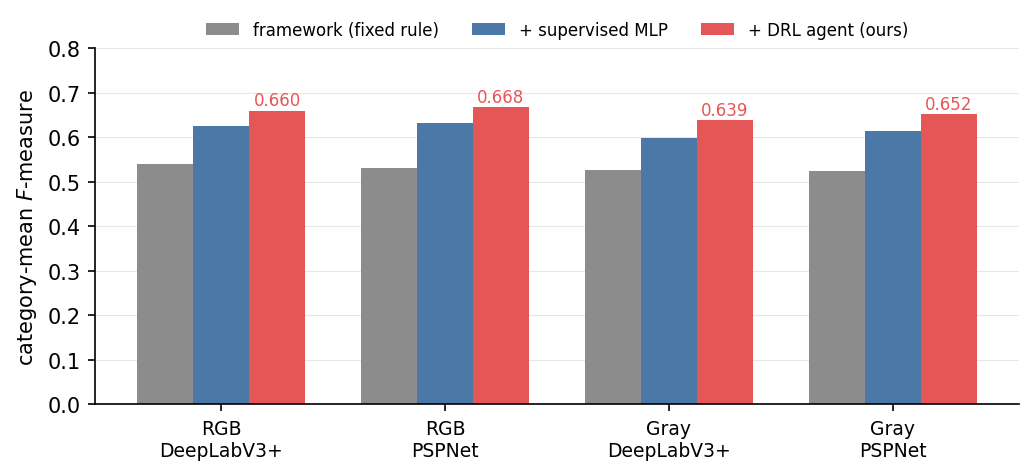
\includegraphics[width=\columnwidth]{fig_robustness_2x2.png}
\caption{Plug-and-play robustness: category-mean \Fm{} across the full $2\times2$ of CPB
representation $\times$ guidance backbone. The learned agent (red) improves the fixed
framework (grey) and the supervised MLP (blue) in every configuration, with a
near-constant margin, evidence that the gain is a property of the learned
arbitration, not of a single pipeline.}
\label{fig:robust}
\end{figure}

%  Table 5: significance 
\begin{table}[t]\centering
\caption{Paired Wilcoxon significance over the $53$ held-out scenes and per-fold gain,
all four configurations. The RL agent beats the supervised control significantly
everywhere, with a near-constant category-mean margin.}
\label{tab:sig}
\small
\setlength{\tabcolsep}{3.5pt}
\resizebox{\columnwidth}{!}{%
\begin{tabular}{lcccc}
\toprule
 & \multicolumn{2}{c}{agent vs.\ framework} & \multicolumn{2}{c}{agent vs.\ MLP}\\
\cmidrule(lr){2-3}\cmidrule(lr){4-5}
configuration & $\Delta$cat & $p$ & $\Delta$cat & $p$\\
\midrule
RGB / DeepLabV3+  & $+0.120$ & $1.0{\times}10^{-7}$ & $+0.035$ & $3.9{\times}10^{-4}$\\
RGB / PSPNet      & $+0.136$ & $1.6{\times}10^{-7}$ & $+0.036$ & $1.2{\times}10^{-4}$\\
Gray / DeepLabV3+ & $+0.112$ & $3.8{\times}10^{-7}$ & $+0.040$ & $2.2{\times}10^{-4}$\\
Gray / PSPNet     & $+0.128$ & $9.2{\times}10^{-8}$ & $+0.037$ & $5.3{\times}10^{-5}$\\
\bottomrule
\end{tabular}}
\\[3pt]
\footnotesize
All $p$-values are exact two-sided paired Wilcoxon over the 53 held-out scenes; the agent
beats the framework on $42$--$45$ of $53$ scenes and the MLP on $37$--$41$. Per-fold
agent$-$framework gain (category-mean): RGB-DL $+0.138\!\pm\!0.070$; RGB-PSP
$+0.155\!\pm\!0.070$; Gray-DL $+0.126\!\pm\!0.042$; Gray-PSP $+0.141\!\pm\!0.046$.
\end{table}

\subsection{Limitations}
\label{sec:limits}
Four limitations are worth stating plainly. First, our re-implemented base framework
is below the authors' absolute level (Sec.~\ref{sec:repro}); we mitigate this by
making every comparison a controlled, identical-pixel delta, but the absolute numbers
should be read as a re-implementation rather than a state-of-the-art claim. Second,
while the agent improves all $11$ categories in the primary RGB\,/\,DeepLabV3+
configuration, it can still slightly harm an isolated category in a cell where the
static rule is already strong, in grayscale\,/\,DeepLabV3+ that is
\textit{nightVideos} ($-0.026$), the sole regression of the four cells, because
acting on disputes there risks overriding a CPB decision that was already correct; the
keep-baseline action limits but does not eliminate this cost. Third, the benefit of the
learned arbiter is conditional on the guidance branch being the unreliable one in the
target domain. The PSPNet cross-dataset transfer
(Sec.~\ref{sec:transfer-pspnet}) makes this concrete: when PSPNet guidance transfers
strongly to LIMU (scene-mean $0.703$), trusting it is already the best simple policy and
the CDnet-trained agent, though it still beats the supervised control and improves the
base, falls below guidance-alone ($0.670$ RGB, $0.684$ grayscale). The cause is that the
agent, having converged to a degenerate keep-baseline rate of $\approx0.00$ on CDnet
 cannot defer to a branch that happens to be excellent on the target. A transfer that
re-enables keep-baseline when both branches are locally confident, or a small amount of
target-domain calibration of the action prior, is the natural remedy and is left to
future work. Fourth, all policies are trained with a single random seed ($1234$); our
significance tests and the four-configuration study address scene and configuration
variability, but not the variability of retraining the policy itself, so the
RL-over-supervised margin should be read as established across scenes and configurations
rather than across training randomness. A multi-seed study is left to future work.

% ============================================================================
\section{Conclusion}
\label{sec:conc}
We revisited the model-communication framework for cross-scene foreground
segmentation and identified its static arbitration rule as the key rigidity. By
learning a lightweight per-pixel policy that acts only on the small set of disputed
pixels (typically well under $10\%$), and by giving that policy a keep-baseline action that preserves the
framework's own Stage-2/3 resolution, we improved our re-implemented
framework's category-mean \Fm{} on CDnet2014 by $+0.11$ to $+0.14$ across a full
$2\times2$ of CPB representations and guidance backbones (primary RGB\,/\,DeepLabV3+:
$0.540\!\rightarrow\!0.660$, all $11$ categories improved), with a tight per-fold
spread. As a reference comparison, on the pooled aggregation consistent with the authors'
published ``Overall'' the full system reaches $0.775$ versus their $0.753$, though on the
stricter category-mean it remains below their computable level, the delivered gain,
not an absolute state-of-the-art claim, is our contribution. Controlled studies, a
single-harness supervised-vs-RL head-to-head, cross-dataset transfer to LIMU, and a
full base$\times$backbone robustness sweep, place the contribution precisely: it is
the \emph{learned, context-aware} arbitration that matters, and, under the matched
three-way action architecture and identical input, reinforcement learning is
\emph{significantly} better at it than a capacity-matched supervised control in all four
configurations ($p$ from $5\times10^{-5}$ to $4\times10^{-4}$), with a near-constant
$+0.037$ category-mean margin, so the arbiter is plug-and-play and robust across the
representation and backbone variants we evaluated. The transfer study also delimits when the
learned arbiter helps: under DeepLabV3+ guidance, which transfers weakly to LIMU, the
agent is the best deployable system, whereas under a PSPNet backbone that itself
transfers strongly it beats the supervised control but falls below guidance-alone 
the benefit is conditional on the guidance branch being the unreliable one in the target
domain, and we trace the residual loss to a degenerate keep-baseline rate; whether a
small transfer-time calibration can remedy this without target labels is left to future
work rather than claimed here. The controlled methodology, faithful re-implementation, identical-pixel
comparison, head-to-head, transfer, and backbone generalisation, offers a template for
evaluating learned components inside classical vision pipelines. A particularly promising
direction is to extend learned arbitration beyond the disputed set to the pixels on which
the two branches \emph{agree yet are jointly wrong}: the present method leaves all agreed
pixels untouched, but a learned policy that also identifies and corrects confident-but-wrong
agreements could recover errors that no disputed-pixel arbiter can reach. Further
directions include reviving the keep-baseline action under strong backbones and
extending the method to further guidance backbones and datasets. A temporal-consistency
reward that couples decisions across frames is also promising: a genuinely sequential
formulation could give reinforcement learning a structural edge over the one-step
decision studied here.



%% ============================================================================
\backmatter

\bmhead{Statements and Declarations}

\noindent\textbf{Funding.} This work was supported by the National Natural Science
Foundation of China under Grant No.~62172217.

\medskip\noindent\textbf{Competing interests.} The authors declare that they have no
known competing financial interests or personal relationships that could have appeared
to influence the work reported in this paper.

\medskip\noindent\textbf{Ethics approval and consent to participate.} Not applicable.
This study does not involve human participants or animals.

\medskip\noindent\textbf{Consent for publication.} Not applicable.

\medskip\noindent\textbf{Data availability.} The CDnet2014 and LIMU datasets used in
this study are publicly available from their respective providers.

\medskip\noindent\textbf{Code availability.} The source code, configurations, and
trained checkpoints will be released on a public repository upon publication.

\medskip\noindent\textbf{Author contributions.}
S.~Gahouidi Junior Thierry: conceptualization, methodology, software, investigation,
formal analysis, validation, visualization, and writing of the original draft.
Z.~Chen: supervision, conceptualization, and writing, review and editing.
All authors read and approved the final manuscript.

\medskip\noindent\textbf{Use of AI-assisted technologies.}
During the preparation of this work the authors used an AI-based assistant for language
editing and formatting only. After using this tool, the authors reviewed and edited the
content as needed and take full responsibility for the content of the manuscript.

%% ============================================================================
\section*{References}
\small
\begin{enumerate}\itemsep1pt
\item[{[1]}] Liang D, Kang B, Liu X, Gao P, Tan X, Kaneko S (2021) Cross-scene foreground segmentation with supervised and unsupervised model communication. Pattern Recognit 117:107995
\item[{[2]}] Liang D, Kaneko S, Hashimoto M, Iwata K, Zhao X (2015) Co-occurrence probability-based pixel pairs background model for robust object detection in dynamic scenes. Pattern Recognit 48(4):1374--1390
\item[{[3]}] Chen LC, Zhu Y, Papandreou G, Schroff F, Adam H (2018) Encoder-decoder with atrous separable convolution for semantic image segmentation. In: Proc Eur Conf Comput Vis (ECCV)
\item[{[4]}] Zhao H, Shi J, Qi X, Wang X, Jia J (2017) Pyramid scene parsing network. In: Proc IEEE Conf Comput Vis Pattern Recognit (CVPR)
\item[{[5]}] Wang Y, Jodoin PM, Porikli F, Konrad J, Benezeth Y, Ishwar P (2014) CDnet 2014: an expanded change detection benchmark dataset. In: Proc IEEE Conf Comput Vis Pattern Recognit Workshops (CVPRW)
\item[{[6]}] Han J, Yang L, Zhang D, Chang X, Liang X (2018) Reinforcement cutting-agent learning for video object segmentation. In: Proc IEEE Conf Comput Vis Pattern Recognit (CVPR)
\item[{[7]}] Williams RJ (1992) Simple statistical gradient-following algorithms for connectionist reinforcement learning. Mach Learn 8:229--256
\item[{[8]}] Zhou B, Zhao H, Puig X, Fidler S, Barriuso A, Torralba A (2017) Scene parsing through ADE20K dataset. In: Proc IEEE Conf Comput Vis Pattern Recognit (CVPR)
\item[{[9]}] Stauffer C, Grimson WEL (1999) Adaptive background mixture models for real-time tracking. In: Proc IEEE Conf Comput Vis Pattern Recognit (CVPR)
\item[{[10]}] Barnich O, Van Droogenbroeck M (2011) ViBe: a universal background subtraction algorithm for video sequences. IEEE Trans Image Process 20(6):1709--1724
\item[{[11]}] St-Charles PL, Bilodeau GA, Bergevin R (2015) SuBSENSE: a universal change detection method with local adaptive sensitivity. IEEE Trans Image Process 24(1):359--373
\item[{[12]}] Babaee M, Dinh DT, Rigoll G (2018) A deep convolutional neural network for video sequence background subtraction. Pattern Recognit 76:635--649
\item[{[13]}] Lim LA, Keles HY (2018) Foreground segmentation using convolutional neural networks for multiscale feature encoding (FgSegNet). Pattern Recognit Lett 112:256--262
\item[{[14]}] Tezcan MO, Ishwar P, Konrad J (2020) BSUV-Net: a fully-convolutional neural network for background subtraction of unseen videos. In: Proc IEEE Winter Conf Appl Comput Vis (WACV)
\item[{[15]}] Braham M, Pi\'erard S, Van Droogenbroeck M (2017) Semantic background subtraction. In: Proc IEEE Int Conf Image Process (ICIP)
\item[{[16]}] Zeng D, Zhu M (2018) Combining background subtraction algorithms with convolutional neural network. J Electron Imaging 27:013011
\item[{[17]}] Jacobs RA, Jordan MI, Nowlan SJ, Hinton GE (1991) Adaptive mixtures of local experts. Neural Comput 3(1):79--87
\item[{[18]}] Shazeer N, Mirhoseini A, Maziarz K, Davis A, Le Q, Hinton G, Dean J (2017) Outrageously large neural networks: the sparsely-gated mixture-of-experts layer. In: Proc Int Conf Learn Represent (ICLR)
\item[{[19]}] Hofmann M, Tiefenbacher P, Rigoll G (2013) Multi-sensor background subtraction by fusing multiple region-based probabilistic classifiers. Pattern Recognit Lett 34(10):1109--1116
\item[{[20]}] Tsai YH, Hung WC, Schulter S, Sohn K, Yang MH, Chandraker M (2018) Learning to adapt structured output space for semantic segmentation. In: Proc IEEE Conf Comput Vis Pattern Recognit (CVPR)
\item[{[21]}] Hoffman J, Tzeng E, Park T, Zhu JY, Isola P, Saenko K, Efros AA, Darrell T (2018) CyCADA: cycle-consistent adversarial domain adaptation. In: Proc Int Conf Mach Learn (ICML)
\item[{[22]}] Wang D, Shelhamer E, Liu S, Olshausen B, Darrell T (2021) Tent: fully test-time adaptation by entropy minimization. In: Proc Int Conf Learn Represent (ICLR)
\item[{[23]}] Finn C, Abbeel P, Levine S (2017) Model-agnostic meta-learning for fast adaptation of deep networks. In: Proc Int Conf Mach Learn (ICML)
\item[{[24]}] Shaban A, Bansal S, Liu Z, Essa I, Boots B (2017) One-shot learning for semantic segmentation. In: Proc Br Mach Vis Conf (BMVC)
\item[{[25]}] Caicedo JC, Lazebnik S (2015) Active object localization with deep reinforcement learning. In: Proc IEEE Int Conf Comput Vis (ICCV)
\item[{[26]}] Yun S, Choi J, Yoo Y, Yun K, Choi JY (2017) Action-decision networks for visual tracking with deep reinforcement learning. In: Proc IEEE Conf Comput Vis Pattern Recognit (CVPR)
\item[{[27]}] Schulman J, Wolski F, Dhariwal P, Radford A, Klimov O (2017) Proximal policy optimization algorithms. arXiv:1707.06347
\item[{[28]}] Haarnoja T, Zhou A, Abbeel P, Levine S (2018) Soft actor-critic: off-policy maximum entropy deep reinforcement learning with a stochastic actor. In: Proc Int Conf Mach Learn (ICML)
\item[{[29]}] Laboratory for Image and Media Understanding (LIMU), Kyushu University. Detection of moving objects dataset
\item[{[30]}] Efron B, Tibshirani R (1993) An Introduction to the Bootstrap. Chapman \& Hall, New York
\item[{[31]}] Kirillov A, Mintun E, Ravi N, Mao H, Rolland C, Gustafson L, Xiao T, Whitehead S, Berg AC, Lo WY, Doll\'ar P, Girshick R (2023) Segment Anything. In: Proc IEEE Int Conf Comput Vis (ICCV)
\item[{[32]}] Wang Q, Fink O, Van Gool L, Dai D (2022) Continual test-time domain adaptation. In: Proc IEEE Conf Comput Vis Pattern Recognit (CVPR)
\item[{[33]}] Tezcan MO, Ishwar P, Konrad J (2021) BSUV-Net 2.0: spatio-temporal data augmentations for video-agnostic supervised background subtraction. IEEE Access 9:53849--53860
\item[{[34]}] An Y, Zhao X, Yu T, Guo H, Zhao C, Tang M, Wang J (2023) ZBS: zero-shot background subtraction via instance-level background modeling and foreground selection. In: Proc IEEE Conf Comput Vis Pattern Recognit (CVPR)
\item[{[35]}] Pokala PK, Pandey NK, Patibandla JSK, Pailla BR (2024) MUSTAN: multi-scale temporal context as attention for robust video foreground segmentation. arXiv:2402.00918
\item[{[36]}] Xie J, Yang C, Xie W, Zisserman A (2024) Moving object segmentation: all you need is SAM (and flow). In: Proc Asian Conf Comput Vis (ACCV)
\item[{[37]}] Huang N, Xie W et al (2025) Segment any motion in videos. In: Proc IEEE Conf Comput Vis Pattern Recognit (CVPR)
\end{enumerate}


\end{document}
